\setcounter{chapter}{0}

\boilerplatechapterone{

The JEOD \ModelDesc gives an extensible framework for specifying general
models of vehicle surface geometry. These models can then be converted to
``interaction specific" (applying to only one type of environmental interaction,
such as aerodynamic or radiation forces) surface models. The extensible
framework allows for new methods of modeling the general surface geometry
to be implemented, as well as allowing for extension to any other
user specified interaction.

The \ModelDesc can either be made up of individual components that remain
fixed with respect to the vehicle structure, or it can have
components that are allowed to move with respect to the vehicle structure.
This optional ability to move components with respect to the vehicle structure
is accomplished by defining position and orientation
of surface model components with respect to atomic mass components in
a mass tree \cite{dynenv:MASS}. The mass tree can then be updated, and
the surface model will update its own geometry accordingly. This feature
can be used to model any vehicle surface feature that will change with respect
to time, such as the articulation of solar arrays or the movements of
a robotic arm.
} {
   \ModelHistory
}

%----------------------------------
\chapter{Product Requirements}\hyperdef{part}{reqt}{}\label{ch:reqt}
%----------------------------------
This chapter will describe the requirements for the \ModelDesc.

\requirement{Top-level requirement}
\label{reqt:toplevel}
\begin{description}
\item[Requirement:]\ \newline
  This model shall meet the JEOD project requirements specified in
  the \JEODid\
  \hyperref{file:\JEODHOME/docs/JEOD.pdf}{part1}{reqt}{ top-level
  document}.
\item[Rationale:]\ \newline
  This model shall, at a minimum,  meet all external and internal requirements 
  applied to the \JEODid\ release.
\item[Verification:]\ \newline
     Inspection
\end{description}   


\requirement{Geometric Modeling}\label{reqt:surfacemodel_geom_modeling}
\begin{description}
\item[Requirement:]\ \newline
The \ModelDesc shall supply a method for representing the geometry
of a vehicle surface.
\item[Rationale:]\ \newline
The basic requirement of the surface model is to represent the geometry
of a vehicle, and this representation is useful in orbital simulations.
\item[Verification:]\ \newline
The verification for this item shall be done by inspection.
\end{description}
 
 \requirement{Environmental Interaction}\label{reqt:surfacemodel_inter_modeling}
 \begin{description}
 \item[Requirement:]\ \newline
 The \ModelDesc shall supply functionality for interactions
 between the surface of a vehicle and its environment.
 \item[Rationale:]\ \newline
 Environmental interactions with the vehicle are necessary for orbit
 simulations, and a geometrical surface model can aid in the calculation
 of these interactions.
 \item[Verification:]\ \newline
 The verification for this item shall be done by a demonstration test.
 \end{description}
 
 \requirement{Extensible Geometrical Modeling}\label{reqt:surfacemodel_exten_geom_modeling}
 \begin{description}
 \item[Requirement:]\ \newline
 The \ModelDesc shall create an extensible method for modeling
 the geometry of a surface.
 \item[Rationale:]\ \newline
 Users may want to specify new and unforseen methods for modeling a surface.
 The framework should be able to handle this.
 \item[Verification:]\ \newline
 The verification for this item shall be done by a demonstration test.
 \end{description}
 
 \requirement{Extensible to Environmental Interactions }\label{reqt:surfacemodel_interaction_extension}
 \begin{description}
 \item[Requirement:]\ \newline
 The \ModelDesc shall be extendable to different environmental
 interactions.
 \item[Rationale:]\ \newline
 The \ModelDesc should be useful in the context of many different
 environmental interactions, including those specified by the end user.
 \item[Verification:]\ \newline
 The verification for this item shall be done by a demonstration test.
 \end{description}
 
 \requirement{Re-use of Models}\label{reqt:surfacemodel_surface_reuse}
 \begin{description}
 \item[Requirement:]\ \newline
 One surface model representation of a vehicle shall be useable with
 many different environmental interactions at the same time.
 \item[Rationale:]\ \newline
 The user should not have to recreate the same geometrical surface model
 in the same simulation to be used with different environmental
 interactions.
 \item[Verification:]\ \newline
 The verification for this item shall be done by a demonstration test.
 \end{description}

 \requirement{Articulation}\label{reqt:surfacemodel_artic}
 \begin{description}
 \item[Requirement:]\ \newline
 The Surface Model shall provide the ability to make its
geometry consistent with the geometry embodied in a mass tree.
 \item[Rationale:]\ \newline
 The Surface Model geometry, if consistent with a mass tree's, would then
 reflect any changes made to the mass tree geometry, allowing for
 changing Surface Model geometry including articulation and other
 movements.
 \item[Verification:]\ \newline
 The verification for this item shall be done testing.
 \end{description}

%% Format for the model Requirements is open.  It should include requirements for this model 
%% only and use requirment tags like the one below.
% \requirement{...}
% \label{reqt:...}
% \begin{description}
%   \item[...]\ \newline
%     The documentation for the model shall include
% 
%     \subrequirement{}
%     \label{reqt:...}
%       Software requirements specification.
%       
%     ...
%    
%   \item[title]\ \newline
%     text
% 
%   ...
%
%\end{description}

%----------------------------------
\chapter{Product Specification}\hyperdef{part}{spec}{}\label{ch:spec}
%----------------------------------

\section{Conceptual Design}

The JEOD \ModelDesc is designed to give an extensible framework
for both describing the geometry of a vehicle, as well as calculating
environmental interactions with that geometry. 

First, a geometry only surface is specified, using 
what this model refers to as ``facets". These facets are
a very general concept and can accomodate any user defined
representation of a part of a vehicle. One example is the FlatPlate
representation described below, which models a part of the vehicle as
a flat surface with only an area, position, and normal vector from the surface.

Then, from this pure geometry
representation, an ``interaction-specific" surface
model can be created. This interaction
specific version will share the geometry of the surface it is created from,
but with the added functionality of calculating some user defined
environmental interaction
such as aerodynamics or radiation pressure.

This design gives many advantages to the end user:

\begin{itemize}
\item{Allows different interaction models to be created from the same
basic surface model},
\item{Allows for complete extensibility of the basic surface model,}
\item{Allows the interaction specific surface models to be extended to
any user defined interaction.}
\end{itemize}

Each facet found in a surface model will - in an interaction specific
surface model created from that geometric model - have an interaction
specific equivalent facet. This equivalent will know everything about
the original geometric Facet, but will also have the ability to
calculate a specific interaction's effects on itself. 

This interaction specific facet is created from the original facet,
using interaction facet specific parameters specified by the
user at runtime, through use of an interaction facet factory,
a concept that will be described below.
An illustration of this process can be seen below in Figure
\ref{fig:facet_flow}.

\begin{figure}[H]
\begin{center}
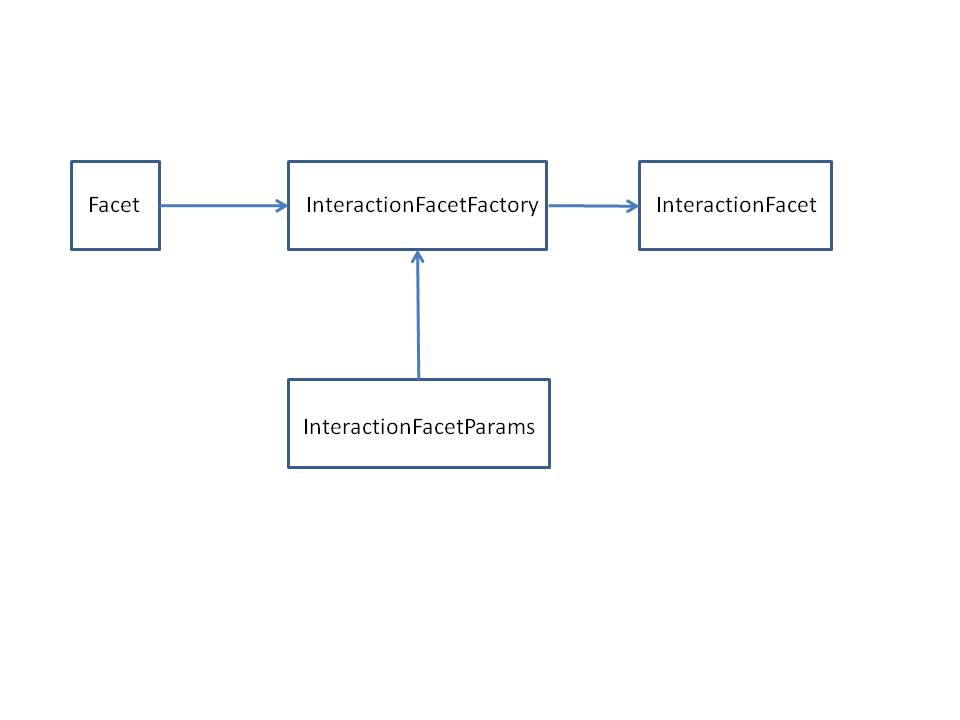
\includegraphics[height=75mm]{figs/facet_flow.jpg}
\caption{An interaction specific facet is created from a general facet,
using a set of facet parameters}
\label{fig:facet_flow}
\end{center}
\end{figure}

The process shown in Figure \ref{fig:facet_flow} is encapsulated within
an interaction surface factory, which creates an interaction
specific surface from a general surface. This interaction surface factory
will be loaded  at runtime by the user with the 
appropriate interaction facet factories and facet parameter objects
necessary to fully create the interaction specific surface
from the original geometry only surface model. An illustration of
this process can be seen below in Figure \ref{fig:surface_flow}.

\begin{figure}[H]
\begin{center}
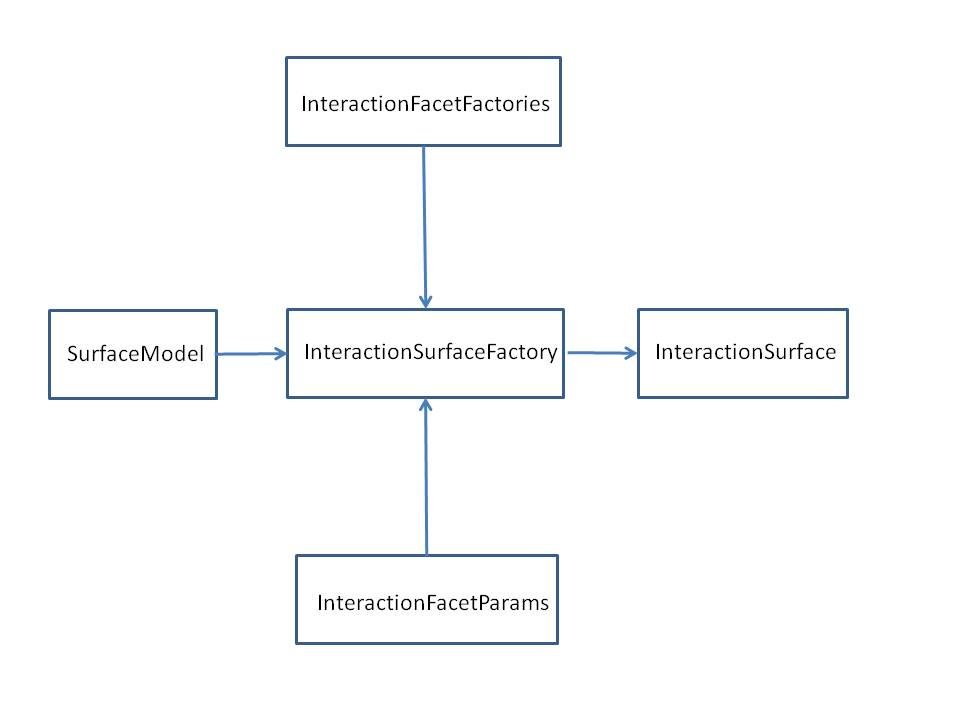
\includegraphics[height=75mm]{figs/surface_flow.jpg}
\caption{An interaction specific surface is created from a general surface,
using a set of facet parameters and interaction facet factories}
\label{fig:surface_flow}
\end{center}
\end{figure}

The \ModelDesc can be split into three parts:

\begin{itemize}
\item{General Surface Geometry Classes},
\item{Interaction Specific Classes}, and
\item{Factory Classes}, those that create interaction specific classes from
general surface geometry classes.
\end{itemize}

The following sections will describe these groups of classes.

\subsection{General Surface Geometry Classes}

This section will describe the classes associated with establishing a general
surface geometry.

\subsubsection{Facet}

The Facet class is the basic building block of the surface model geometry.
A Facet specifies actual geometry of a vehicle. How big of a slice of geometry
a Facet represents is up to the user; a single
facet can be a complete representation of a
vehicle, or just a small component. This gives flexibility to the end user in how
they wish to represent the geometry of the vehicle. 

Facet geometry can be described in two ways. One option is the specifying the
geometry directly in the user desired structural frame of the vehicle.
The facet geometry can also be
specified relative to the structural reference frame inherently contained
in a user supplied MassBody object \cite{dynenv:MASS}, thus tying
each facet in the model to a MassBody in a mass body tree. In this second case,
the position and orientation of the facet in the user desired structural frame
will then be calculated, where the desired structural frame is
defined as being the structural frame of a MassBody object in the same
mass body tree as the one tied to the facet. This allows for re-positioning
of facets relative to one another or to the structural reference frame during run time,
merely by adjusting the relative states of MassBodys in the mass body tree.
Note that the articulation option is only available for Facet (and classes
deriving from Facet) that have been specifically designed to support
articulation. Currently, the only JEOD supplied Facet that supports
articulation is the FlatPlate class. However, a user can
add articulation to any Facet derived type
simply by inheriting from the type and implementing the
correct functions, as described in the Users Guide of this
document.

Additional flexibility is
given because Facet is intended to be a base class for other classes, thus
it can be derived from and have user desired parameters attached to it. An
example of this is FlatPlate, described momentarily, which inherits from
the Facet class and adds its own necessary parameters. Thus, new types
of facets can be created by inheriting from Facet. Creating facets in
this way is the suggested usage when using the
\ModelDesc.

\subsubsection{SurfaceModel}

The SurfaceModel class represents the complete geometry of a vehicle. It
contains a list of pointers to Facet objects (pointers in order to take advantage
of types inheriting from Facet and that allow multiple types of facets
to be used within the same SurfaceModel object). These individual facets 
make up the
complete geometry of the surface model, and SurfaceModel is thus a containing
class for a list of Facet derived objects.

\subsubsection{FlatPlate}

The FlatPlate class is an inheriting object from Facet. It represents a flat
plate form of surface geometry, and includes information about the flat plate's
area and normal vector.

The FlatPlate class inherits from the Facet class, and fully implements
all Facet functionality. Its geometry can be specified either
in a user defined structural frame, or using the interface to a
MassBody tree
as described in the Facet class description and in the Users Guide
of this document.

\subsubsection{FlatPlateThermal}

The FlatPlateThermal class extends the FlatPlate class with the
Thermal-Rider Model \cite{dynenv:THERMALRIDER}. Further information
about this functionality can be found in the appropriate documentation.

\subsubsection{SurfaceModelMessages}

The SurfaceModelMessages class enumerates messages associated with
warnings and failures of the \ModelDesc.

\subsection{Interaction Specific Classes}

The interaction specific classes of the \ModelDesc are designed to mirror
the pure geometry classes, while adding information and functionality
associated with a specific ``interaction." Interaction in this usage refers
to a specific environmental interaction with the vehicle, such as aerodynamics
or radiation pressure, however, it can refer to anything that will succesfully
fit into the presented framework.

\subsubsection{InteractionFacet}

The InteractionFacet is the interaction specific equivalent of the Facet class.
For any particular interaction desiring to use the Surface Model, an
InteractionFacet inheriting class will be created. Interaction specific
equivalent classes for facet types (classes inheriting from the Facet
class) can then be created. 

For example, the JEOD Aerodynamics model
\cite{dynenv:AERODYNAMICS} creates an InteractionFacet inheriting class
AeroFacet, which adds the pure virtual functionality for calculating
aerodynamic forces. Then, a new class is inherited from AeroFacet,
FlatPlateAeroFacet, which is the aerodynamic interaction equivalent
of flat plate. When an aerodynamic interaction specific surface model
is created from a surface model containing a flat plate facet, the
aerodynamic specific surface model will contain a FlatPlateAeroFacet
equivalent for each FlatPlate object found in the original SurfaceModel.

\subsubsection{InteractionSurface}

The InteractionSurface class is a pure virtual base class that defines
the interface for interaction specific surface models. 
Any new interaction that is meant to interact with the \ModelDesc will
create an interaction specific class inheriting from InteractionSurface.
This inheriting class will then contain an
array of pointers to the appropriate class that inherits from
InteractionFacet, and this array will then be populated when
the interaction surface is created from a base SurfaceModel
object.

An example of this inheritance can be found in the JEOD Aerodynamics
Model \cite{dynenv:AERODYNAMICS}. AeroSurface inherits from
InteractionSurface, and contains an array of pointers to
AeroFacet objects. These pointers will then be populated with
the correct type of aerodynamic specific interaction facets when
the AeroSurface is created from a SurfaceModel object.

\subsubsection{FacetParams}

The FacetParams class is a base class for specifying interaction
specific parameters that are necessary when creating an interaction specific
facet. A user will inherit from FacetParams, populating the
class with parameters necessary for the specific facet type and interaction
in question. These parameters will then be used to create the
InteractionFacet from the Facet, and will be matched to facets in 
a SurfaceModel object by name lookup. These parameters are especially
useful for values associated with a specific type of interaction facet
that need to be specified by the user at runtime.

\subsection{Factory Classes}

This section will describe the classes used to create
both specific interaction surfaces from general surfaces, as well as
specific interaction facets from general facets.

\subsubsection{InteractionSurfaceFactory}

The InteractionSurfaceFactory is a utility class that creates
an interaction specific surface model from a basic, geometry only
surface model. It is meant to be a base class for an interaction specific
surface factory, creating surfaces for a particular interaction from
base SurfaceModel objects. These objects are able to, given the correct
inputs, create their specific interaction surface models from a base
SurfaceModel object.

\subsubsection{InteractionFacetFactory}

The InteractionFacetFactory is a pure virtual class. It creates an interface
for classes which will take a specific Facet type (such as FlatPlate), and
create from it an interaction specific version of that Facet (for
the aerodynamics interaction, a FlatPlate will be turned into a 
FlatPlateAeroFacet, an aerodynamic specific version of FlatPlate).
These classes will be vital utility classes for the InteractionSurfaceFactory, which will create an interaction specific surface from a basic
geometric surface by creating interaction specific facets from
all of the basic surface's facets.

\subsection{Additional Classes}

There are additional classes found in the Surface Model directory, such as PlatePolygon, PlateEllipse, and others.
While these files are found in the Surface Model directory, they are mainly Facet derived classes
created for the JEOD Contact Model \cite{dynenv:CONTACT}. Please see the appropriate  documentation for additional
information, and note that these Facet derived classes do not support the articulation feature of the
Surface Model.

\section{Mathematical Formulations}

There is no accompanying mathematical formulation for the \ModelDesc.
All mathematical formulations will occur in interaction specific 
implementations of the surface model. Examples of this can be seen in
the Aerodynamics Model \cite{dynenv:AERODYNAMICS} and the Radiation Pressure
Model \cite{dynenv:RADIATIONPRESSURE}.

\section{Detailed Design}

The complete API for the \ModelDesc can be found
in the  \href{file:refman.pdf} {\em Reference Manual}
\cite{surfacemodelbib:ReferenceManual}.

\clearpage
\boilerplateinventory

%----------------------------------
\chapter{User Guide}\hyperdef{part}{user}{}\label{ch:user}
%----------------------------------
The Instructions for Simulation Users section of the user guide is intended primarily for users of pre-existing simulations.  
It contains: 
\begin{itemize}
\item A description of how to modify \ModelDesc variables after the simulation 
has compiled, including an in-depth discussion of the input file,
\item An overview of how to interpret (but not edit) the S\_define file,
\item A sample of some of the typical variables that may be logged.
\end{itemize}

The Instructions for Simulation Developers section of the user guide is intended for simulation developers.  
It describes the necessary configuration of the \ModelDesc within an 
S\_define file, and the creation of standard run directories.  The latter 
component assumes a thorough understanding of the preceding Analysis section of the user guide.
Where applicable, the user may be directed to selected portions of Product Specification (Chapter \ref{ch:spec}).

The Instructions for Model Developers section of the user guide is intended primarily for developers 
needing to extend the capability of the \ModelDesc.  Such users should have a 
thorough understanding of how the model is used in the preceding 
Integration section, and of the model 
specification (described in Chapter \ref{ch:spec}).

\section{Instructions for Simulation Users}

For this section, the following S\_define object will be
assumed:

\begin{verbatim}
sim_object { 

   utils/surface_model: SurfaceModel surface;
   utils/surface_model: DemoSurface inter_surface;
   utils/surface_model: DemoSurfaceFactory surf_fact;

   unsigned int integer;

   /* Scheduled Jobs */
   utils/surface_model: Facet ** facet_ptr;

   utils/surface_model: DemoFacet * demo_facet;

   (0.0, environment) utils/surface_model:
   surface_model.surface.add_facets(
      In Facet** new_facets = surface_model.facet_ptr,
      In unsigned int num_new_facets = surface_model.integer);

   utils/surface_model: DemoParams * dp1;

   utils/surface_model: FacetParams * facet_params;

   (0.0, environment) utils/surface_model:
   surface_model.surf_fact.add_facet_params(
      In FacetParams* to_add = surface_model.facet_params);

   // These are only here so trick can see them. they are not
   // used otherwise.
   utils/surface_model: DemoFacetFactory dff;


   utils/surface_model: InteractionFacetFactory * facet_factory;
   (0.0, environment) utils/surface_model:
   surface_model.surf_fact.add_facet_factory(
      In InteractionFacetFactory* to_add = surface_model.facet_factory
      );

   (initialization) utils/surface_model:
   surface_model.surf_fact.create_surface(
      In SurfaceModel* surface = &surface_model.surface,
      Out InteractionSurface* inter_surface = &surface_model.inter_surface);

} surface_model;
\end{verbatim}

There are a variety of theoretical objects in this sim\_object, used
for demonstration purposes. They are:

\begin{itemize}
\item{DemoSurface}, a class inheriting from InteractionSurface, meant
to interact with a theoretical interaction class,
\item{DemoSurfaceFactory}, a class inheriting from InteractionSurfaceFactory,
\item{DemoFacet}, a class inheriting from Facet,
\item{DemoFacetFactory}, a class inheriting from InteractionFacetFactory
that creates an interaction facet (DemoInteractionFacet), 
representing the theoretical
interaction specific version of DemoFacet,
\item{DemoParams}, a FacetParams derived object used to create
a DemoInteractionFacet from a DemoFacet through use of a DemoFacetFactory. 
\end{itemize}

Note that, for JEOD supplied interaction models such as Aerodynamics
\cite{dynenv:AERODYNAMICS} and Radiation Pressure
\cite{dynenv:RADIATIONPRESSURE}, a thorough explanation of using
those interactions with the \ModelDesc is contained
in the respective model's documentation, and should be consulted.

There are two options for creating facets that are then added to the SurfaceModel
object:

\begin{itemize}
\item{statically allocating them, either in a user defined object or directly in
the S\_define, or}
\item{dynamically allocating them either in code or in the input file.}
\end{itemize}

If the facets are statically allocated, then the user must simply add them
to the instantiated SurfaceModel using either the
`add\_facets' or `add\_facet' SurfaceModel member functions, as shown
in the API document \cite{surfacemodelbib:ReferenceManual}.

If the user dynamically allocates the facets in code, and the user requires
the simulation to be fully checkpointable, then the user is responsible
to use the appropriate methods through Trick to insure that the facets
are checkpointable. This is not an inherent requirement of the surface model, and
is only necessary if the user requires checkpointing.

The user can also allocate facets in the input file. The following
section demonstrates this procedure.

\subsection{Allocating Facets}

This section demonstrates allocating
facets in the input file. While this User Guide mainly focuses on a Trick 7
implementation (as a Trick 10 implementation is mostly analagous),
care must be taken in allocating facets in Trick 10 such that they will
be fully accessible and checkpointable by Trick. Thus, this section
will give specific examples of both.

The example S\_define presented in the previous section will
be used for the Trick 7 demonstration. The Trick 10 demonstration will
use its own.

\subsubsection{Allocating Facets in Trick 7}

In Trick 7, dynamic allocation of facets can be done
through the following code:

\begin{verbatim}
#define NUM_DEMO_FACETS 2 // Two for example purposes only

DemoFacet** temp_demo_facets;
temp_demo_facets = alloc(NUM_DEMO_FACETS);
temp_demo_facets[0] = new DemoFacet[1];
temp_demo_facets[1] = new DemoFacet[1];

temp_demo_facets[0]->parameter = demo_value;
temp_demo_facets[1]->parameter = other_demo_value;

temp_demo_facets[0]->name = "demo_facet";
temp_demo_facets[1]->name = "demo_facet";

temp_demo_facets[0]->param_name = "demo_params";
temp_demo_facets[1]->param_name = "demo_params";

surface_model.facet_ptr = temp_demo_facets;
surface_model.integer = NUM_DEMO_FACETS;

call surface_model.surface_model.surface.add_facets(surface_model.facet_ptr);
\end{verbatim}

This code snippet will allocate the DemoFacet objects to be added to
the SurfaceModel object, populate them with the appropriate values
associated with that particular class (demonstrated here by populating
the member values ``parameter" with ``demo\_value" and ``other\_demo\_value")
and calling the function to dynamically add the newly allocated DemoFacets
to the SurfaceModel. This procedure may be repeated any number of times,
to add any type of Facet inherited objects to the SurfaceModel object
that the user wishes.

Next, the appropriate parameters used to create the DemoInteractionFacet
objects from the DemoFacet objects must be allocated, populated and
added to the DemoSurfaceFactory. This can be done with the following
code snippet:

\begin{verbatim}

DemoParams* params;
params = new DemoParams;
params->parameter = example_value;

params->name = "demo_params";

surface_model.facet_params = params;

call surface_model.surface_model.surf_fact.add_facet_params(
   surface_model.facet_params);

\end{verbatim}

This example allocates a set of DemoParams, populates them, and
adds them to the surface factory that will be responsible for creating
the DemoInteractionFacet from the DemoFacet. This procedure may be
done for as many FacetParams inheriting params as is necessary to create
the corresponding InteractionFacet inherited objects from all
Facet derived objects that were added to the surface model.

Note that the DemoFacet object has a field called ``param\_name", and
DemoParams has a field called ``name."
It is these name fields that the DemoSurfaceFactory
will use to match the parameters that are loaded onto it with the
Facet inherited objects it finds in the SurfaceModel object supplied
to it. If a correctly named FacetParams inherited object is not found
for a particular Facet inherited object found in the SurfaceModel, then
a message will be sent through the JEOD Message Handler
\cite{dynenv:MESSAGE} and a failure will occur.

Finally, the InteractionFacetFactory objects necessary for
creating the DemoSurface object from the supplied SurfaceModel object
must be added to the InteractionSurfaceFactory subclass DemoSurfaceFactory.
This can be done with the following code
snippet:

\begin{verbatim}
DemoFactory* = df;
df = new DemoFactory;

surface_model.facet_factory = df;

call surface_model.surface_model.surf_fact.add_facet_factory(
   surface_model.facet_factory);
\end{verbatim}

Care must be taken that, for every type of Facet added to the SurfaceModel
above, an appropriate InteractionFacetFactory inherited class that is
also appropriate for the Interaction at hand, must be added to
the InteractionSurfaceFactory. If this is not done then the
initialization of the InteractionSurface will fail, as the
InteractionSurfaceFactory will find a Facet that it does not know how
to handle.

The InteractionSurface derived class DemoSurface may now be used in
the appropriate, user defined manner.

\subsubsection{Allocating Facets in Trick 10}

The steps for dynamically allocating facets in the input file in Trick 10 are
mostly analogous to those used in Trick 7. Outside of a few minor and noted
details, the procedure is the same, with only syntactic resulting in the input file.

These examples will rely heavily on built in utilities provided to the user by Trick.
A thorough understanding of the input file, as it applies to Trick 10, are
recommended, and the Trick 10 documentation on that subject should be well understood.

To demonstrate this, the following
example S\_define will be used:

\begin{verbatim}
##include "utils/surface_model/verif/include/demo_facet.hh"
##include "utils/surface_model/verif/include/demo_factory.hh"
##include "utils/surface_model/verif/include/demo_interaction.hh"
##include "utils/surface_model/verif/include/demo_interaction_facet.hh"
##include "utils/surface_model/verif/include/demo_params.hh"
##include "utils/surface_model/verif/include/demo_surface.hh"
##include "utils/surface_model/verif/include/demo_surface_factory.hh"


class SurfaceModelSimObject : public Trick::SimObject {

public:

   // Objects
   SurfaceModel surface;
   DemoSurface inter_surface;
   DemoSurfaceFactory surf_fact;

   // Pointers used for dynamic allocation
   DemoFacet* demo_facet; 
   DemoParams* demo_params;
   DemoFactory* demo_factory;


   SurfaceModelSimObject() 
   {
      
   ("initialization") surf_fact.create_surface(&surface, &inter_surface);

   }

};

// Instantiate the surface model sim object.
SurfaceModelSimObject surface_model;
\end{verbatim}

The zero rate jobs (`add\_facets', `add\_facet\_params' and `add\_facet\_factory') as seen
in the earlier Trick 7 version are no longer necessary, as member functions can now be called from
the input file without registering them as a job with Trick. Also, it is necessary to include the definition
of any type of facet intended to be allocated through a Trick `\#\#include' declaration.

If the allocated facets need to be checkpointable, the following Python code can be used for allocation:

\begin{verbatim}
surface_model.demo_facet = trick.alloc_type(1, "DemoFacet")
# A temporary reference to the facet to save typing
temp_facet = surface_model.demo_facet
temp_facet.parameter = demo_value
temp_facet.param_name = "demo_params"
surface_model.surface.add_facet(temp_facet)
\end{verbatim}

This code allocates a single facet, fills out
the appropriate values, then adds it to the SurfaceModel
object. This differs slightly from the Trick 7 version, in that
it is much easier to add facets one at a time in Trick 10.
Note the use of the intermediate pointer `surface\_model.demo\_facet,'
which is of type DemoFacet*. This is necessary
for Python to be able to correctly type the returned value from `trick.alloc\_type.'

If the ability to checkpoint is not a requirement, then the following code
can instead be used:

\begin{verbatim}
temp_facet = trick.DemoFacet()
temp_facet.thisown = 0
temp_facet.parameter = demo_value
temp_facet.param_name = "demo_params"
surface_model.surface.add_facet(temp_facet)
\end{verbatim}

A similar pattern is followed to allocate the facet parameter objects and 
the interaction surface factories. For the case where checkpointing is required:

\begin{verbatim}
surface_model.demo_params = trick_alloc_type(1, "DemoParams")
# A temporary reference to the params to save typing
temp_params = surface_model.demo_params
temp_params.parameter = example_value
surface_model.surface.add_facet_params(temp_params)
\end{verbatim}

For the case where checkpointing is not required:

\begin{verbatim}
temp_params = trick.DemoParams()
temp_params.thisown = 0
params.parameter = example_value
surface_model.surface.add_facet_params(temp_params)
\end{verbatim}

Similarly, allocating checkpointable interaction facet factories can be
done using the following code:

\begin{verbatim}
surface_model.demo_factory = trick.alloc_type(1, "DemoFactory")
# A temporary reference to the factory to save typing
temp_factory = surface_model.demo_factory
surface_model.surface.add_factory(temp_factory)
\end{verbatim}

If checkpointing is not a requirement:

\begin{verbatim}
temp_factory = trick.DemoFactory()
temp_factory.thisown = 0
surface_model.surface.add_factory(temp_factory)
\end{verbatim}

\subsection{Specifying Facet Geometry}

There are two possible ways to specify geometry of a facet:

\begin{itemize}
\item{Specifying the geometry directly in the desired frame, usually the structural frame
of the represented vehicle, or}
\item{Specifying the geometry with respect to a MassBody's structural frame, through the
articulation interface.}
\end{itemize}

The following sections will describe both of these methods.

\subsubsection{Specifying Geometry Directly in the Desired Frame}

The first, and easiest, method for specifying facet geometry is
to specify it directly in the user desired frame, most commonly
the structural frame of the represented vehicle.

In the case of a FlatPlate, the position and the normal direction
can be specified directly by setting the parameters ``position" and
``normal," as shown below:

\begin{verbatim}
FlatPlate flat_plate;

flat_plate.position[0] {M} = 5.0,  2.0,   1.0;
flat_plate.normal[0] = 1.0 , 0.0 , 0.0; 
\end{verbatim}

This command places the flat plate at the position noted,
with a normal completely in the ``X" direction, with respect to
the frame implicitely chosen by the user.

Note that the variables being set are ``position" and ``normal".
These are fundamentally different than the corresponding 
``local\_position" and ``local\_normal". These ``local\_" versions
of the variables are only for use when the articulation
capability is in use. If the user wishes
to directly set the normal and position in their choosen frame,
this example should be followed and the ``local\_" versions
should be left untouched.

Also note that, when using this method, JEOD does not enforce a specific
frame for specifying facet geometry. While the vehicle structural frame
is the most common (as seen both in the Aerodynamics \cite{dynenv:AERODYNAMICS}
and Radiation Pressure \cite{dynenv:RADIATIONPRESSURE} interaction
models), this is not enforced. Additionally, this frame
is never explicitely set, and is only implicit based on the
user's intent. It is up to the user to
ensure that all facets in a surface model are represented with respect
to a common frame, and that it is the frame that other models
using the surface model are expecting.

Finally, it should be noted that any interaction model that is using a surface
model, for a FlatPlate or any Facet inheriting the ``position" attribute,
should only access these variables. The ``local\_" versions of these variables
are not intended to be used as an output, and should be treated as such.

\subsubsection{Specifying Geometry through the Articulation Interface}

The second way a user can specify the geometry of a Facet is
by connecting Facets to MassBody objects in a mass tree, through
the provided articulation interface. This section will describe
this method. This section will rely heavily on knowledge of the JEOD
Mass Model and its documentation \cite{dynenv:MASS}.

This method allows the user to attach a Facet to a movable reference frame, where a ``global"
position and orientation for that reference frame will automatically be calculated by the surface
model. This is accomplished by attaching all Facets to frames associated with individual
mass bodies in a tree, as well as specifying a single ``output frame" for the global
position and orientation.

In this method of specifying geometry, each Facet is specified with respect
to the structural reference frame of a specific mass body. This differs
from the method described in the previous section, where all facets
were specified in a common, user defined implicit frame. For example,
this specification is done for a FlatPlate by setting the following
variables:

\begin{verbatim}
FlatPlate flat_plate;

flat_plate.local_position[0] {M} = 5.0,  2.0,   1.0;
flat_plate.local_normal[0] = 1.0 , 0.0 , 0.0; 
\end{verbatim}

Note that this is different than the previous example, as instead of
``position" and ``normal," the variables being set are
``local\_position" and ``local\_normal". 

The specified position and normal
is relative to the structural frame of a particular mass body. The
user specifies which mass body by name, as in the following
example:

\begin{verbatim}
flat_plate.mass_body_name = "name_of_mass_body";
\end{verbatim}

This name must match that of a mass body contained in the
mass tree of the vehicle this surface represents. For details
on making sure this name is correct, as usual, see the
MassBody documentation \cite{dynenv:MASS}.

Next, the user must tell the surface model which mass body
structural frame will be the ``global" frame, by naming the 
associated mass body in the following manner:

\begin{verbatim}
SurfaceModel surface;
surface.struct_body_name = "name_of_struct_body";
\end{verbatim}

As with the Facet's ``mass\_body\_name," this name must correspond to the
name of a mass body in the mass tree of the vehicle this surface
represents. Additionally, the named mass must be in the same mass tree
as all of the named masses associated with all of the Facets in the
surface model. If this is not true then the articulation component
will throw a failure message through the JEOD Message Handler
\cite{dynenv:MESSAGE}.

The Facet geometry, specified in this manner, is meant to be static with
respect to the Facet's specified mass body. Once the articulation feature
of the surface model is invoked, the appropriate transformations
will be applied to this specified geometry to represent the position
and orientation of the Facet in the structural frame
of the mass body that is named by SurfaceModel's ``struct\_body\_name". For a FlatPlate,
this information will then be stored in the ``position" and ``normal" variables.
As mentioned in the previous section, these are the variables that should then
be accessed by an interaction model using this surface.

Finally, the user must turn on the articulation feature, using the
following code as an example:

\begin{verbatim}
surface.articulation_active = true;
\end{verbatim}

Note that this is set to false by default.

This association to a mass body then allows for articulation by movement of
mass bodies, within the tree, relative to one another. For details on
moving mass bodies relative to one another in a tree, see the appropriate
documentation \cite{dynenv:MASS}.

Please note that, at this time, the only Facet derived type that supports this articulation
feature is the FlatPlate. Any other Facets supplied by JEOD will have undefined behavior
if they are used in association with the articulation feature. For any other user created
Facets, check with the individual developer to see if the correct functionality has been implemented.

Additionally, the articulation feature will only work if the correct functionality has been
placed in the S\_define. Details for this can be found in the Integration section of this document.

\section{Instructions for Simulation Developers}

This section will be broken into two versions, one for simulation development in Trick 7 and
one for Trick 10.

\subsection{Simulation Development in Trick 7}

This section will use the following S\_define object as an example:

\begin{verbatim}
sim_object { 

   utils/surface_model: SurfaceModel surface;
   utils/surface_model: DemoSurface inter_surface;
   utils/surface_model: DemoSurfaceFactory surf_fact

   unsigned int integer;

   utils/surface_model: Facet ** facet_ptr;

   utils/surface_model: DemoFacet * demo_facet;

   (0.0, environment) utils/surface_model:
   surface_model.surface.add_facets(
      In Facet** new_facets = surface_model.facet_ptr,
      In unsigned int num_new_facets = surface_model.integer);

   utils/surface_model: DemoParams * dp1;

   utils/surface_model: FacetParams * facet_params;

   (0.0, environment) utils/surface_model:
   surface_model.surf_fact.add_facet_params(
      In FacetParams* to_add = surface_model.facet_params);

   // These are only here so Trick can see them. they are not
   // used otherwise.
   utils/surface_model: DemoFacetFactory dff;


   utils/surface_model: InteractionFacetFactory * facet_factory;
   (0.0, environment) utils/surface_model:
   surface_model.surf_fact.add_facet_factory(
      In InteractionFacetFactory* to_add = surface_model.facet_factory
      );

   (initialization) utils/surface_model:
   surface_model.surf_fact.create_surface(
      In SurfaceModel* surface = &surface_model.surface,
      Out InteractionSurface* inter_surface = &surface_model.inter_surface);

} surface_model;
\end{verbatim}

This section will also use the same theoretical SurfaceModel
classes, for demonstration purposes, as found in the
Analysis section.

Note that, for JEOD supplied interaction models such as Aerodynamics
\cite{dynenv:AERODYNAMICS} and Radiation Pressure
\cite{dynenv:RADIATIONPRESSURE}, a thorough explanation of using
those interactions with the \ModelDesc is contained
in the respective model's documentation, and should be consulted.

First, a basic surface model object and a surface model appropriate
for the specific interaction at hand must be instantiated. Additionally,
the surface factory necessary to populate the interaction surface must
be instantiated. This is shown in the following S\_define snippet:

\begin{verbatim}
   utils/surface_model: SurfaceModel surface;
   utils/surface_model: DemoSurface inter_surface;
   utils/surface_model: DemoSurfaceFactory surf_fact;
\end{verbatim}

Next, the hooks for dynamically allocating the Facet derived objects
and adding them to the SurfaceModel object through an input file are
added:

\begin{verbatim}  

   unsigned int integer;

   utils/surface_model: Facet ** facet_ptr;

   utils/surface_model: DemoFacet * demo_facet;

   (0.0, environment) utils/surface_model:
   surface_model.surface.add_facets(
      In Facet** new_facets = surface_model.facet_ptr,
      In unsigned int num_new_facets = surface_model.integer);
    
\end{verbatim}

Note that the DemoFacet pointer ``demo\_facet" is never legitimately
used. It is only included so that Trick is aware of its existence
and so that it can be dynamically allocated in the input file.
This inclusion of all Facet derived types that will be added
in the input file that uses this S\_define is necessary, or the
dynamic allocation will not work, and must be done by the Integrator
that is creating the S\_define.

Next, the hooks to dynamically add FacetParams derived objects
must be added to the S\_define using the following code:

\begin{verbatim}
   utils/surface_model: DemoParams * dp1;

   utils/surface_model: FacetParams * facet_params;

   (0.0, environment) utils/surface_model:
   surface_model.surf_fact.add_facet_params(
      In FacetParams* to_add = surface_model.facet_params);
\end{verbatim}

Similar to the DemoFacet pointer described above, the DemoParams
pointer seen here is never used. It is only necessary for Trick
awareness. An inclusion in the S\_define of this type is
necessary for every type of FacetParams derived object that will be
used with this particular S\_define, or the dynamic allocation of that
particular type in the input file will be unsuccessful.

Next, the hooks to dynamically add InteractionFacetFactory derived
objects to the DemoSurfaceFactory must be added, using the following
code:

\begin{verbatim}
   utils/surface_model: DemoFacetFactory* dff;

   utils/surface_model: InteractionFacetFactory * facet_factory;

   (0.0, environment) utils/surface_model:
   surface_model.surf_fact.add_facet_factory(
      In InteractionFacetFactory* to_add = surface_model.facet_factory
      );
\end{verbatim}

Once again, the DemoFacetFactory pointer is never used, and is only
present to make Trick aware of the type so that dynamic allocation in the
input file is possible.

Finally, the DemoSurface must be created from the SurfaceModel, using
the following code:

\begin{verbatim}
   (initialization) utils/surface_model:
   surface_model.surf_fact.create_surface(
      In SurfaceModel* surface = &surface_model.surface,
      Out InteractionSurface* inter_surface = &surface_model.inter_surface);
\end{verbatim}

The DemoSurface has now been populated and is ready for use 
with the appropriate interaction model.


\subsection{Simulation Development in Trick 10}

The following S\_define example will be used to demonstration simulation development in Trick 10.
This is a similar example to that used in the previous Trick 10 example of allocating checkpointable
facets in the input file, and the same usage will be assumed.

\begin{verbatim}
##include "utils/surface_model/verif/include/demo_facet.hh"
##include "utils/surface_model/verif/include/demo_factory.hh"
##include "utils/surface_model/verif/include/demo_interaction.hh"
##include "utils/surface_model/verif/include/demo_interaction_facet.hh"
##include "utils/surface_model/verif/include/demo_params.hh"
##include "utils/surface_model/verif/include/demo_surface.hh"
##include "utils/surface_model/verif/include/demo_surface_factory.hh"


class SurfaceModelSimObject : public Trick::SimObject {

public:

   // Objects
   SurfaceModel surface;
   DemoSurface inter_surface;
   DemoSurfaceFactory surf_fact;

   // Pointers used for dynamic allocation, when checkpointing is necessary
   DemoFacet* demo_facet; 
   DemoParams* demo_params;
   DemoFactory* demo_factory;


   SurfaceModelSimObject() 
   {
      
   ("initialization") surf_fact.create_surface(&surface, &inter_surface);

   }

};

// Instantiate the surface model sim object.
SurfaceModelSimObject surface_model;
\end{verbatim}

Because of Python's ability to directly call object member functions from the input file, the S\_define
in Trick 10 is slightly cleaner.

The first thing a developer must do is include all definitions for objects that will be instantiated
in the sim object, as well as objects that are intended to be dynamically allocated in the input file,
as `\#\#include' commands, shown in this example as:

\begin{verbatim}
##include "utils/surface_model/verif/include/demo_facet.hh"
##include "utils/surface_model/verif/include/demo_factory.hh"
##include "utils/surface_model/verif/include/demo_interaction.hh"
##include "utils/surface_model/verif/include/demo_interaction_facet.hh"
##include "utils/surface_model/verif/include/demo_params.hh"
##include "utils/surface_model/verif/include/demo_surface.hh"
##include "utils/surface_model/verif/include/demo_surface_factory.hh"
\end{verbatim}

A basic surface model object and an interaction specific surface model, as well
as a surface factory necessary to populate the interaction surface, must be instantiated.
This is demonstrated in the following S\_define snippet:

\begin{verbatim}
   SurfaceModel surface;
   DemoSurface inter_surface;
   DemoSurfaceFactory surf_fact;
\end{verbatim}

If facets are to be allocated dynamically, and the user wishes for them to be checkpointable, then
any allocable types must have an intermediate pointer declared for them in the S\_define, demonstrated
in this code snippet:

\begin{verbatim}
   DemoFacet* demo_facet; 
   DemoParams* demo_params;
   DemoFactory* demo_factory;
\end{verbatim}

This code will allow for types DemoFacet, DemoParams and DemoFactory to be allocated and checkpointable
in the input file. If checkpointing is not a requirement, then these declarations are optional and can
be left out.

Finally, all that is left is to register the initialization job for creating the interaction surface.

\begin{verbatim}
   ("initialization") surf_fact.create_surface(&surface, &inter_surface);
\end{verbatim}

\subsection{Articulation}

There are additional pieces necessary to enable the use of articulation
in an S\_define. The following additional calls, and pieces, should be added:

\begin{verbatim}

sim_object {

   DynManager dyn_manager;

}

sim_object {
   (initialization) utils/surface_model:
   surface_model.surface.initialize_mass_connections(
      In DynManager& manager = mngr.dyn_manager);

   (1.0, environment) utils/surface_model:
      surface_model.surface.update_articulation();
} surface_model;
\end{verbatim}

As usual, this is a partial code snippet only used to illustrate this procedure.

Two jobs must be added to allow use of the articulation feature. The first is an
initialization job, which will use the DynManager interface to connect all
Facets to their appropriate mass bodys, as described in the Analysis section of this document.
This job is called ``initialize\_mass\_connections," and must be supplied with a DynManager
object. This object must be pre-loaded with all masses (or MassBody derived objects, such as
DynBody objects \cite{dynenv:DYNBODY}) that are named by the user, as described in the Analysis section,
for use with the invoking SurfaceModel object.

The second job tells the surface model to update the current ``global" state of all facets. This is a simple
call, as illustrated above, to the ``update\_articulation" function. Once this function has been called,
all updates to the ``global" position and orientation of Facets will have occurred.

All of these instructions are completely analogous for Trick 10, and as a result
a specific Trick 10 example will not be presented. However, the same jobs can merely be
added to a Trick 10 sim object, and will have the same effect.

\section{Instructions for Model Developers}

There are two ways to extend the \ModelDesc. The first is to add
new representations for facets to the geometric surface model. The second
is to extend the surface model to work with other environmental interactions.
Both will be discussed in this section.

\subsection{Extending the Facet Class}

To extend the Facet class, a user must create a new class that inherits from
Facet, and populate it with the required data for the new representation.
Because of the design of the SurfaceModel object (containing an array of
pointers to the Facet base class), this new Facet inherited class can now be
added to a SurfaceModel object.

Note that, to use this new Facet inherited class in an interaction, the
interaction specific version of the surface model will also need to be extended.
This, however, is a part of extending the environmental interaction, and thus
will be covered in the next section.

\subsubsection{Extending the Facet Class for Articulation}

To enable articulation for an extension of the facet class, one protected virtual method must be implemented. This method is:

\begin{verbatim}
virtual void update_articulation_internal();
\end{verbatim}

and is inherited from the Facet class.

When this method is called, the member variable:

\begin{verbatim}
MassPointState mass_rel_struct;
\end{verbatim}

also inherited from the Facet class, will be populated with the relative state between the 
structural frame of the mass body associated
with this particular facet, and the structural frame of the ``global" mass body associated with
the entire surface model, from the global frame to the facet frame. For details of this class,
see the Mass Model documentation \cite{dynenv:MASS}.

The extender must now correctly use this information to transform any user specified local geometry, as determined
by the extender and correctly added to their class, into the ``global" frame, and this information must then be
stored in the extended Facet. How this is done is ultimately left up to the user, and example implementation are found
in both the Facet class and the FlatPlate class.

Note that, for the ``position" parameter found in all Facet classes, the Facet version of this function can be called
explicitly from the extended version, using the call:

\begin{verbatim}
Facet::update_articulation_internal();
\end{verbatim}

Additionally, an extender inheriting from the FlatPlate class can also call the FlatPlate version to update both the global position
and normal.

Note that it may be advantageous to a user, if one is not intending for a particular Facet derived class to be used for articulation,
for the extender to explicitly override this function, and have the function issue information to the user through the JEOD
Message Handler. Details on this can, of course, be found in the appropriate documentation \cite{dynenv:MESSAGE}.

\subsection{Extending to New Environmental Interactions}

Extending the \ModelDesc to new environmental classes involves creating
a variety of subclasses to take advantage of the architecture of the
\ModelDesc. This section will describe the steps that must be taken.

Note that both the JEOD Aerodynamics Model \cite{dynenv:AERODYNAMICS} and the
Radiation Pressure Model \cite{dynenv:RADIATIONPRESSURE} extend the
\ModelDesc for their own use, and these models serve as examples
for the information that will be given here.

For the purpose of demonstration, an interaction called ``NewInteraction" will
be supposed. This is, obviously, illustrative only.

The first step is to create a subclass of InteractionFacet particular to the
new interaction. This subclass is what will actually be contained
in the eventual NewInteraction specific InteractionSurfaceModel class, and
will, through virtual functionality, dictate the API for the calculation
of ``NewInteraction". An example of this is the class AeroFacet 
\cite{dynenv:AERODYNAMICS}, which inherits from InteractionFacet and adds
the pure virtual function shown below:

\begin{verbatim}
virtual void aerodrag_force(
   const double velocity_mag,
   const double rel_vel_hat[3],
   AeroDragParameters* aero_drag_param_ptr, 
   double center_grav[3]) = 0;
\end{verbatim}

This now gives the InteractionFacet class implicit aerodrag functionality.
A similar path should be taken for the ``NewInteraction". The extender
should create an InteractionFacet inherited class (hypothetically called
``NewInteractionFacet") and add the pure virtual
function that will be responsible for calculating the new interaction's effects
on all interaction facets contained in the model.

Next, the user must create a specific subclass of InteractionSurfaceModel
for the new interaction. This new class, hypothetically called 
``NewInteractionSurfaceModel," will contain an array of pointers to the
previously created ``NewInteractionFacet." An example of this
inheritance is the AeroSurface class found in the Aerodynamics Model
\cite{dynenv:AERODYNAMICS}.

Additionally, two functions must be implemented in the 
``NewInteractionSurfaceModel" class; ``allocate\_array" and
``allocate\_interaction\_facet." These are pure virtual functions
in the InteractionSurface class, and there is standard code that can
be used to implement them in a ``NewInteractionSurfaceModel" class. 
The follow code snippet, intended for a header file, will help illustrate
this concept.

\begin{verbatim}
   NewInteractionFacet** inter_facets;

   unsigned int facets_size; /* cnt Size of the inter_facets array */

   // Allocates the inter_facets array from the given size
   virtual void allocate_array (unsigned int size);

   // Allocates the facet at the "index" value in inter_facets, using
   // the base Facet given by the pointer facet, and using the parameter
   // object pointed to by params pointer and using the
   // InteractionFacetFactory pointed to by factory.
   virtual void allocate_interaction_facet (
      Facet* facet,
      InteractionFacetFactory* factory,
      FacetParams* params,
      unsigned int index);
\end{verbatim}

Given this code snippet, the code for the pure virtual functions can be implemented in
the following manner.

\begin{verbatim}
void
NewInteractionSurface::allocate_array ( // Return: -- void
   unsigned int size) // In: cnt: The size of the needed array
{

   if (inter_facets != nullptr) {
      // USE THE JEOD MESSAGE HANDLER TO SEND A FAILURE MESSAGE.
      return;
   }

   // Allocate the array we want, and set the size
   inter_facets = JEOD_ALLOC_CLASS_POINTER_ARRAY (size, AeroFacet);
   facets_size = size;

   // Make sure all pointers are NULL so destructor never crashes
   for (unsigned int ii = 0; ii < facets_size; ++ii) {
      aero_facets[ii] = nullptr;
   }

   return;

}

void
AeroSurface::allocate_interaction_facet ( // Return: -- void
   Facet* facet, /* In: -- The basic facet used to create the
                           interaction facet */
   InteractionFacetFactory* factory, /* In: -- The factory used to create
                                           the interaction facet */
   FacetParams* params, /* In: -- The aero params used to create the
                              interaction facet */
   unsigned int index) /* In: cnt Where the new interaction facet will be placed
                              in the aero_facets array */
{
   if (facets_size <= index) {


      // SEND A MESSAGE USING THE JEOD MESSAGE HANDLER
      return;

   }

   /* need to temporarily save off the InteractionFacet returned before
      dynamic casting it. If the dynamic cast fails, we want to destroy
      the InteractionFacet so we don't get a memory leak */

   InteractionFacet* temp_facet = nullptr;

   // attempt to create the facet
   temp_facet = factory->create_facet (facet, params);

   // if the facet is nullptr, then we have a problem
   if (temp_facet == nullptr) {

      // SEND A MESSAGE USING THE JEOD MESSAGE HANDLER

   }

   // Facet is currently an interaction facet. Try to make it a
   // NewInteractionFacet

   NewInteractionFacet* temp_inter_facet = 
      dynamic_cast<NewInteractionFacet*> (temp_facet);


   // If that fails, it doesn't belong in this surface so there is a problem
   if (temp_inter_facet == nullptr) {

      // temp_facet can NOT be NULL, since it was already checked for above
      JEOD_DELETE_OBJECT (temp_facet);

      // SEND A MESSAGE THROUGH THE JEOD MESSAGE HANDLER


      return;

   }

   // Store the aero_facet into the aero_facets array
   inter_facets[index] = temp_inter_facet;

   return;

}
\end{verbatim}

This prepares the NewInteractionSurface class to succesfully allocate its
own array of InteractionFacet derived objects, as well as populate an
index of that array given a correct Facet pointer, InteractionFacetFactory
pointer and FacetParams pointer.

Additionally, to prevent a memory leak, the allocated array of
NewInteractionFacet pointers and their allocated memory must be
deleted by the destructor of this new class. Example code for doing this
can be seen below:

\begin{verbatim}
NewInteractionSurface::~NewInteractionSurface (
   void)
{

   if (inter_facets != nullptr) {

      for (unsigned int ii = 0; ii < facets_size; ++ii) {
         if (inter_facets[ii] != nullptr) {
            JEOD_DELETE_OBJECT (aero_facets[ii]);
         }
      }

      JEOD_DELETE_ARRAY (inter_facets);

   }

}
\end{verbatim}

Note that references are made in these code snippets 
to the JEOD Message Handler
\cite{dynenv:MESSAGE}. These messages will involve interaction model
specific messages, and need to be written by the user themself. Additional
information can be found in the Message Handler documentation. Additionally,
references are made to JEOD alloc and delete functions. Details on this
functionality can be found in the JEOD Memory utility
\cite{dynenv:MEMORY}.

Next, a subclass of FacetParams should be created that defines a
NewInteraction specific set of parameters. While this is not a necessary
step, it insures type safety when working with the \ModelDesc.
This inherited class, theoretically called ``NewInteractionParams," can be
empty.

Next, an interaction specific class inheriting from
InteractionSurfaceFactory must be created. Like the creation of the
NewInteractionParams, this insures type safety. This new class,
theoretically called ``NewInteractionSurfaceFactory" will have one
function implemented:

\begin{verbatim}
   virtual void add_facet_params (FacetParams* to_add);
\end{verbatim}

This function will check that the FacetParams pointer is of an object
of the correct type (i.e. inheriting from NewInteractionParams), then
add the FacetParams object to the surface factory through the already
existing SurfaceFactory function of the same name. Example code
for this is as follows:

\begin{verbatim}

void
NewInteractionSurfaceFactory::add_facet_params (
   FacetParams* to_add)
{

   if ((to_add->name == NULL) || (to_add->name[0] == '\0')) {

      // SEND A FAILUTRE MESSAGE THROUGH THE MESSAGE HANDLER

   }

   // The param MUST be an
   NewInteractionParams* temp_ptr = nullptr;

   temp_ptr = dynamic_cast<NewInteractionParams*> (to_add);

   if (temp_ptr == nullptr) {

      // SEND A MESSAGE THROUGH THE MESSAGE HANDLER
      return;
   }

   // Add the parameter through the inherited function
   InteractionSurfaceFactory::add_facet_params (to_add);

   return;

}
\end{verbatim}

Finally, a set of classes must be created for every basic type of geometric facet
(in other words, class that inherits from the Facet class) the extender
wants to make available to the new interaction. Three classes will be created,
inheriting from:

\begin{itemize}
\item{NewInteractionFacet}, which will be the NewInteraction specific version
of the particular Facet subclass at hand,
\item{InteractionFacetFactory}, the class that will be responsible for creating
the interaction specific version of the facet from the facet itself, and
\item{NewInteractionParams}, the parameters necessary to create the
NewInteractionFacet subclass from the Facet subclass (typically NewInteraction
specific values necessary for the calculation of the interaction).
\end{itemize}

For illustrative purposes, the remainder of this section will assume that
the extender wishes to use the FlatPlate representation of Facet in
the NewInteraction already being discussed. Obviously the Surface Model
can be extended to any Facet subclass following these instructions, but FlatPlate
will be used as the example.

The extender would create
three classes:

\begin{itemize}
\item{NewInteractionFlatPlate}, a version of flat plate, inheriting from
NewInteractionFacet, that knows how to calculate the effects of NewInteraction
on itself,
\item{NewInteractionFlatPlateParams}, parameters necessary to the
NewInteractionFlatPlate class to calculate the new interaction effects on
the flat plate, and
\item{NewInteractionFlatPlateFactory}, inheriting from InteractionFacetFactory
and with the ability to create a NewInteractionFlatPlate from a FlatPlate
given the correct parameters.
\end{itemize}

The NewInteractionFlatPlate class inherits from NewInteractionFacet. It will contain
all data necessary for calculating the new interaction effect on the flat plate
in question. Also, the extender will have to implement the pure virtual function
created in NewInteractionFacet, as described earlier. This implementation should
calculate the interaction effects on the flat plate itself. If force and torque
are a product of the interaction then these results can be stored in the
appropriately named variables that have been inherited from the
InteractionFacet class. Once the data members have been added and the
pure virtual function implemented, the NewInteractionFlatPlate is ready
for use in the \ModelDesc.

The NewInteractionFlatPlateParams object is simple to create. Inheriting
from NewInteractionParams, the extender can add any parameters necessary for
calculating the new interaction's effects on a flat plate that must be
set at run time by the user. Once the class has been created and the parameters
added to it, the NewInteractionFlatPlateParams class is ready to be used in the
\ModelDesc.

The NewInteractionFlatPlateFactory class, inheriting from InteractionFacetFactory,
is responsible for creating a NewInteractionFlatPlate from a FlatPlate.
To do this, two functions must be implemented in the NewInteractionFlatPlateFactory
class:

\begin{verbatim}
   virtual bool is_correct_factory (Facet* facet);

   virtual InteractionFacet* create_facet (Facet* facet, FacetParams* params);

\end{verbatim}

These are functions inherited from InteractionFacetFactory, where they are
pure virtual.

The ``is\_correct\_factory" function is simple to create. Given a pointer to a Facet
(usually pointing to an object of a Facet subclass), the
function returns a true if the pointer is to an object that the
class was meant to work on, and false otherwise. This function can be
easily programmed using a simple pattern, shown below for the case of
the NewInteractionFlatPlateFactory class.

\begin{verbatim}
bool
NewInteractionFlatPlateFactory::is_correct_factory (
   Facet* facet)
{

   // Simple. do a typeid, if it is true return true, otherwise
   // return false.
   if (typeid(*facet) == typeid(FlatPlate)) {
      return true;
   }
   else {
      return false;
   }

}
\end{verbatim}

The ``create\_facet" function takes in a Facet pointer and a FacetParams
pointer, and returns a pointer to an allocated InteractionFacet.
Taking advantage of polymorphism, the Facet pointer is most commonly
pointing to a subclass of Facet, and the FacetParams pointer is
pointing to a subclass of FacetParams. Type-checking is done at
a variety of levels: the Facet is checked to insure that it is
the correct Facet subclass associated with this particular
InteractionFacetFactory, and the FacetParams is checked for the
same criteria. Once these steps are both taken, the NewInteractionFlatPlate
object will be created, populated with the parameters found in
the NewInteractionFlatPlateParams object sent in, and return the
new object. Example of this complete function can be found
in the following code snippet:

\begin{verbatim}
InteractionFacet*
FlatPlateAeroFactory::create_facet (
   Facet* facet,
   FacetParams* params)
{

   NewInteractionFlatPlateParams* inter_params = nullptr;
   FlatPlate* flat_plate            = nullptr;

   inter_params = dynamic_castNewInteractionFlatPlateParams*> (params);
   flat_plate  = dynamic_cast<FlatPlate*> (facet);

   // We have tried casting the facet and params to the correct types.
   // if they were not the correct type, send out an error message

   if (inter_params == nullptr) {

      // SEND A MESSAGE THROUGH THE MESSAGE HANDLER
   }
   if (flat_plate == nullptr) {

      // SEND A MESSAGE THROUGH THE MESSAGE HANDLER
   }

   // Create the interaction facet
   NewInteractionFlatPlate* inter_facet =
      JEOD_ALLOC_CLASS_OBJECT (NewInteractionFlatPlate, ());


   // Fill it out from the parameters and from the facet itself
   inter_facet->base_facet = facet;

   // Populate the NewInteractionFlatPlate with the parameters from
   // the passed in NewInteractionFlatPlateParams here. This step
   // is left up to the individual extender, as it will be
   // interaction specific.

   return inter_facet;

}
\end{verbatim}

All pieces are now in place, and the new classes may be used
as described above in the Analysis and Intergration sections.



%----------------------------------
\chapter{Verification and Validation}\hyperdef{part}{ivv}{}\label{ch:ivv}
%----------------------------------


% requirement codes
% reqt:surfacemodel_geom_moeling
% reqt:surfacemodel_inter_modeling
% reqt:surfacemodel_exten_geom_modeling
% reqt:surfacemodel_interaction_extension
% reqt:surfacemodel_surface_reuse

\section{Verification}
%%% code imported from old template structure
%\inspection{<Name of Inspection>}\label{inspect:<label>}
% <description> to satisfy  
% requirement \ref{reqt:<label>}.

\inspection{Top-level inspection}\label{inspect:TLI}
 This document structure, the code, and associated files have been inspected, and together satisfy requirement \traceref{reqt:toplevel}.

\inspection{Geometric Modeling Inspection}\label{inspect:geo_modeling}

The \ModelDesc contains the following fully implemented classes:

\begin{itemize}
\item{Facet}, an extensible class that models one part of a surface,
and
\item{SurfaceModel}, a collection of facets representing a complete
vehicle geometric surface.
\end{itemize}

Thus, by inspection, the \ModelDesc satisfies
requirement \traceref{reqt:surfacemodel_geom_modeling}.


\section{Validation}

\test{Multiple Interaction, Multiple
Facet Demo}\label{surfacemodel_demonstration}
\begin{description}
\item[Purpose:]\ \newline

The purpose of this test is to demonstrate the following:

\begin{itemize}
\item{Extensibility of the geometric representation of the surface model,}
\item{Functionality of the surface model with environmental interactions,}
\item{Usability of a single SurfaceModel object with multiple
environmental interactions,}
\item{Extensibility of the Surface Model to multiple environmental
interactions.}
\end{itemize}

\item[Requirements:]\ \newline
%By passing this test, the universal time module 
%partially satisfies requirement~\ref{reqt:<label1>} and 
%completely satisfies requirement~\ref{reqt:<label2>}.
By passing this test, the \ModelDesc satisfies requirement
\traceref{reqt:surfacemodel_inter_modeling}, requirement
\traceref{reqt:surfacemodel_exten_geom_modeling}, requirement
\traceref{reqt:surfacemodel_interaction_extension}, and requirement
\traceref{reqt:surfacemodel_surface_reuse}.

\item[Procedure:]\ \newline

A set of demonstration test classes were created. These classes
demonstrate a variety of features of the \ModelDesc, and
include:

\begin{itemize}
\item{DemoFacet}, a new subclass of Facet,
\item{DemoInteraction1}, a demonstration interaction meant to interact
with the \ModelDesc,
\item{DemoInteraction2}, a second demonstraction interaction meant
to interact with the \ModelDesc,
\item{DemoSurface1}, a subclass of InteractionSurface specifically
for DemoInteraction1,
\item{DemoSurface2}, a subclass of InteractionSurface specifically
for DemoInteraction2.
\end{itemize}

This is not a complete list of the classes created for this verification;
other utility classes were also created to facilitate the complete
implementation of the \ModelDesc for the new interactions
DemoInteraction1 and DemoInteraction2. Both of these interactions
will ask each interaction facet in their supplied interaction
surface model to execute its interaction specific function, as described
later in this section.

A SurfaceModel object will be created and populated with both a FlatPlate
object and a DemoFacet object. This will demonstrate the extensible
nature of the geometric modeling of the \ModelDesc.

Two surface models, one each for the new interactions DemoInteraction1
and DemoInteraction2, will be created and demonstrated to be usable
with the interactions. This will demonstrate the usefulness of the
\ModelDesc with environmental interactions, as well as
the reusability of a single SurfaceModel object for multiple
environmental interactions. Additionally, it will demonstrate that
the surface model is extensible to many interactions.

The two new interactions will be simple; they will trigger the individual
interaction facet contained within the appropriate interaction facets
contained within the created interaction surfaces. This output will
be triggered through a pure virtual function declared in the
InteractionFacet base classes for each interaction. The InteractionFacet
base class for DemoInteraction1 is ``DemoFacet1", which declares
the pure virtual function:

\begin{verbatim}
virtual void execute_demo_1(
   unsigned int interaction_number
   ) = 0;
\end{verbatim}

where the argument ``interaction\_number" is an integer set in
DemoInteraction1 itself, which will be printed out. This will
demonstrate that the interaction is indeed working with the individual
interaction facets of the interaction surface.

The InteractionFacet base class for DemoInteraction2 is ``DemoFacet2,"
which declares the pure virtual function:

\begin{verbatim}
virtual void execute_demo_2(
   char* interaction_name
   ) = 0;
\end{verbatim}

where the argument ``interaction\_name" is a string set in
DemoInteraction2 itself, which will be printed. This will
demonstrate that the interaction is indeed working with the
individual interaction facets of the interaction surface.

Other information will be printed out during the run of the test.
This information is controlled from the input file, and will serve
to demonstrate the extensibility of the \ModelDesc.

The DemoFacet contains the following parameters:

\begin{verbatim}
char* name;
int some_int;
\end{verbatim}

There are four specific interaction facets in this demonstration:
a DemoInteraction1 specific FlatPlate facet, a DemoInteraction2
specific FlatPlate facet, a DemoInteraction1 specific DemoFacet, and
a DemoInteraction2 specific DemoFacet. These interaction facets
all have parameters set by the user, through FacetParams objects, at
runtime.

The FlatPlateDemo1 (DemoInteraction1 specific FlatPlate) contains:

\begin{verbatim}
char* shape;
\end{verbatim}

The FlatPlateDemo2 (DemoInteraction2 specific FlatPlate) contains:

\begin{verbatim}
int sides;
\end{verbatim}

The DemoInteractionFacet1 (DemoInteraction1 specific DemoFacet) contains:

\begin{verbatim}
double weight;
\end{verbatim}

The DemoInteractionFacet2 (DemoInteraction2 specific DemoFacet) contains:

\begin{verbatim}
char* color;
\end{verbatim}

Both FlatPlateDemo1 and DemoInteractionFacet1 implement the pure
virtual function ``execute\_demo\_1". Their implementations are:

\begin{verbatim}
void FlatPlateDemo1::execute_demo_1 (
   unsigned int interaction_number){
   FlatPlate* base_plate = dynamic_cast<FlatPlate*> (base_facet);

   printf("\n\n\n");
   printf("FlatPlateDemo1::execute_demo_1\n");
   printf("The interaction number is: %d\n", interaction_number);
   printf("The shape is: %s\n", shape);
   printf("Area of flat plate is: %f\n", base_plate->area);
   printf("normal of flat plate is: %f %f %f\n",
      base_plate->normal[0],
      base_plate->normal[1],
      base_plate->normal[2]);

   return;
}

void DemoInteractionFacet1::execute_demo_1 (
   unsigned int interaction_number){
   DemoFacet* base_plate = dynamic_cast<DemoFacet*> (base_facet);
   printf("\n\n\n");
   printf("DemoInteractionFacet1::execute_demo_1\n");
   printf("The interaction number is: %d\n", interaction_number);
   printf("The weight is: %f\n", weight);
   printf("the name of the DemoFacet is: %s\n", base_plate->name);
   printf("the semi-random int of the DemoFacet is: %d\n",
      base_plate->some_int);

}

\end{verbatim}

As can be seen, both implementations print out information supplied
by the interaction itself, the original geometric facet the
interaction facet was created from, and from the interaction facet
itself.

Both FlatPlateDemo2 and DemoInteractionFacet2 implement the pure
virtual function ``execute\_demo\_2." Their implementations are:

\begin{verbatim}
void FlatPlateDemo2::execute_demo_2 (
   char* interaction_name){
   FlatPlate* base_plate = dynamic_cast<FlatPlate*> (base_facet);
   printf("\n\n\n");
   printf("FlatPlateDemo2::execute_demo_2\n");
   printf("The interaction name is: %s\n", interaction_name);
   printf("The number of sides is: %d\n", sides);
   printf("Area of flat plate is: %f\n", base_plate->area);
   printf("normal of flat plate is: %f %f %f\n",
      base_plate->normal[0],
      base_plate->normal[1],
      base_plate->normal[2]);

}

void DemoInteractionFacet2::execute_demo_2 (
   char* interaction_name){
   DemoFacet* base_plate = dynamic_cast<DemoFacet*> (base_facet);
   printf("\n\n\n");
   printf("DemoInteractionFacet2::execute_demo_2\n");
   printf("The interaction name is: %s\n", interaction_name);
   printf("The color is: %s\n", color);
   printf("the name of the DemoFacet is: %s\n", base_plate->name);
   printf("the semi-random int of the DemoFacet is: %d\n",
      base_plate->some_int);

}
\end{verbatim}

Like the implementations of ``execute\_demo\_1," 
both implementations print out information supplied
by the interaction itself, the original geometric facet the
interaction facet was created from, and from the interaction facet
itself.

The following is the input file that is used for this demonstration
test. This input file will dictate what will be expected from the output
of the two interactions.

\begin{verbatim}
// allocate the flat plate and populate it

FlatPlate** temp_flat_plate;
temp_flat_plate = alloc(1);
temp_flat_plate[0] = new FlatPlate[1];

temp_flat_plate[0]->position[0] = 1255.0, 0.0, 383.4;
temp_flat_plate[0]->area = 119.4454385;
temp_flat_plate[0]->normal[0] = 1.0, 0.0, 0.0;
temp_flat_plate[0]->param_name = "flat_plate_material";

// allocate the DemoFacet and populate it

DemoFacet** temp_demo_facet;
temp_demo_facet = alloc(1);
temp_demo_facet[0] = new DemoFacet[1];

temp_demo_facet[0]->name = "demo_basic_facet";
temp_demo_facet[0]->some_int = 1337; // random integer
temp_demo_facet[0]->param_name = "demo_basic_facet";

// load the facets onto the surface

surface_model.facet_ptr = temp_flat_plate;
surface_model.integer = 1;

call surface_model.surface_model.surface.add_facets(
   surface_model.facet_ptr);

surface_model.facet_ptr = temp_demo_facet;

call surface_model.surface_model.surface.add_facets(
   surface_model.facet_ptr);

// facets have now been added to the surface.
// add the facet factories onto the surface factories

// Add the factory to create a FlatPlateDemo1 from a FlatPlate

 FlatPlateDemoFactory1* fpf1_ptr;
 fpf1_ptr = new FlatPlateDemoFactory1;
 
 surface_model.facet_factory = fpf1_ptr;
 
call surface_model.surface_model.surf_fact1.add_facet_factory(
   surface_model.facet_factory);

// Add the factory to create a FlatPlateDemo2 from a FlatPlate

FlatPlateDemoFactory2* fpf2;
fpf2 = new FlatPlateDemoFactory2;

surface_model.facet_factory = fpf2;

call surface_model.surface_model.surf_fact2.add_facet_factory(
   surface_model.facet_factory);

// Add the factory to create a DemoInteractionFacet1 from a DemoFacet

DemoFacetFactory1* dff1;
dff1 = new DemoFacetFactory1;

surface_model.facet_factory = dff1;
 
call surface_model.surface_model.surf_fact1.add_facet_factory(
   surface_model.facet_factory);
 
 // Add the factory to create a DemoINteractionFacet2 from a DemoFacet
 
 DemoFacetFactory2* dff2;
 dff2 = new DemoFacetFactory2;
 
 surface_model.facet_factory = dff2;
 
call surface_model.surface_model.surf_fact2.add_facet_factory(
   surface_model.facet_factory);

// The facet factories have now all been added.
// Now add the params to the facet factories

DemoParams1* params1;
params1 = new DemoParams1;

params1->weight = 3.14;
params1->name = "demo_basic_facet";

surface_model.facet_params = params1;

call surface_model.surface_model.surf_fact1.add_facet_params(
   surface_model.facet_params);

// Add demo params to surface factory 2

DemoParams2* params2;
params2 = new DemoParams2;

params2->color = "burnt orange";
params2->name = "demo_basic_facet";

surface_model.facet_params = params2;

call surface_model.surface_model.surf_fact2.add_facet_params(
   surface_model.facet_params);

// add flat plate demo params to surface factory 1

FlatPlateDemoParams1* fpparams1;
fpparams1 = new FlatPlateDemoParams1;

fpparams1->shape = "octagon";
fpparams1->name = "flat_plate_material";

surface_model.facet_params = fpparams1;

call surface_model.surface_model.surf_fact1.add_facet_params(
   surface_model.facet_params);

// add the flat plate demo params to surface actory 2

FlatPlateDemoParams2* fpparams2;
fpparams2 = new FlatPlateDemoParams2;

fpparams2->sides = 6;
fpparams2->name = "flat_plate_material";

surface_model.facet_params = fpparams2;

call surface_model.surface_model.surf_fact2.add_facet_params(
   surface_model.facet_params);

surface_model.inter1.interaction_number = 24601;
surface_model.inter2.interaction_name = "demonstration interaction";

stop = 0.1;

\end{verbatim}

Running this verification test should output, correctly, the values
defined by the input file, demonstrating the geometric
extensibility, the environmental interaction extensibility, the reusability
of surface models across different interactions, and the successful
use of the surface model for environmental interactions.

\item[Results:]\ \newline

The output from the demonstration test is as follows:

\begin{verbatim}
FlatPlateDemo1::execute_demo_1
The interaction number is: 24601
The shape is: octagon
Area of flat plate is: 119.445438
normal of flat plate is: 1.000000 0.000000 0.000000



DemoInteractionFacet1::execute_demo_1
The interaction number is: 24601
The weight is: 3.140000
the name of the DemoFacet is: demo_basic_facet
the semi-random int of the DemoFacet is: 1337



FlatPlateDemo2::execute_demo_2
The interaction name is: demonstration interaction
The number of sides is: 6
Area of flat plate is: 119.445438
normal of flat plate is: 1.000000 0.000000 0.000000



DemoInteractionFacet2::execute_demo_2
The interaction name is: demonstration interaction
The color is: burnt orange
the name of the DemoFacet is: demo_basic_facet
the semi-random int of the DemoFacet is: 1337
\end{verbatim}

All values match correctly, which makes this a successful demonstration
of the utility of the \ModelDesc.
\end{description}

\test{Basic Articulation Test}\label{test:art_test_0}

\begin{description}

\item[Purpose:] \ \newline
SIM directory: SIM\_ARTICULATION
RUN directory: SET\_test/RUN\_articulation\_0

The purpose of this test is to qualitatively demonstrate the 
basic functionality of the articulation feature.

\item[Requirements:] \ \newline

By passing this test, the \ModelDesc partially satisfies
the requirement \traceref{reqt:surfacemodel_artic}

\item[Procedure:] \ \newline

This is a simple test, used to qualitatively demonstrate that
the articulation feature of the \ModelDesc is behaving
in an expected fashion.

For this demonstration, three mass bodies will be used: A, B and C.
Body A will be a parent to both Body B and Body C; thus
Body B and Body C will be siblings to one another. Initially,
all bodies will have zero relative state, meaning that their
structural frames will be coincident and aligned.

Six FlatPlates will be examined, two connected to each MassBody.
For all MassBodys, the first FlatPlate has a normal pointing in
the positive X direction, and the second FlatPlate has a normal
pointing in the negative X direction. All FlatPlates are positioned
coincident with the structural frame of the MassBody to which
they are attached.

This test runs for 360 seconds. MassBody B will be reoriented with respect to
MassBody A, rotating it around the Z axis with no change in position, at a rate of
one degree per second. This should cause the
normals of the two FlatPlates associated with to make a full rotation in the X-Y plane, with
no change in position.

MassBody C will be re-positioned with respect to MassBody A. The
functions used to reposition are as follows:

\begin{equation}\label{position_equation_1}
x = t
\end{equation}
\begin{equation}\label{position_equation_2}
y = -t
\end{equation}
\begin{equation}\label{position_equation_3}
z = 2 * t
\end{equation}

\item[Results:] \ \newline

The following items are expected to always hold their nominal value.

\begin{itemize}
\item{All FlatPlate 1 attributes},
\item{All FlatPlate 2 attributes},
\item{FlatPlate 3's local and global position},
\item{FlatPlate 4's local and global position},
\item{FlatPlate 5's local and global normal},
\item{FlatPlate 6's local and global normal}.
\end{itemize}

All of these values have been checked, and it has been verified that they hold
their nominal values throughout the simulation.

FlatPlate 3's local normal is completely in the X direction. Thus, if MassBody B
rotates in the Z direction relative to , it is expected that FlatPlate's local normal will
remain stationary, but the ``global" normal will rotate through the X-Y plane, in a
counter-clockwise manner, returning to its original position at the end of the
simulation. This behavior is shown below in Figure \ref{fig:artic_normal_3}.

\begin{figure}[H]
\begin{center}
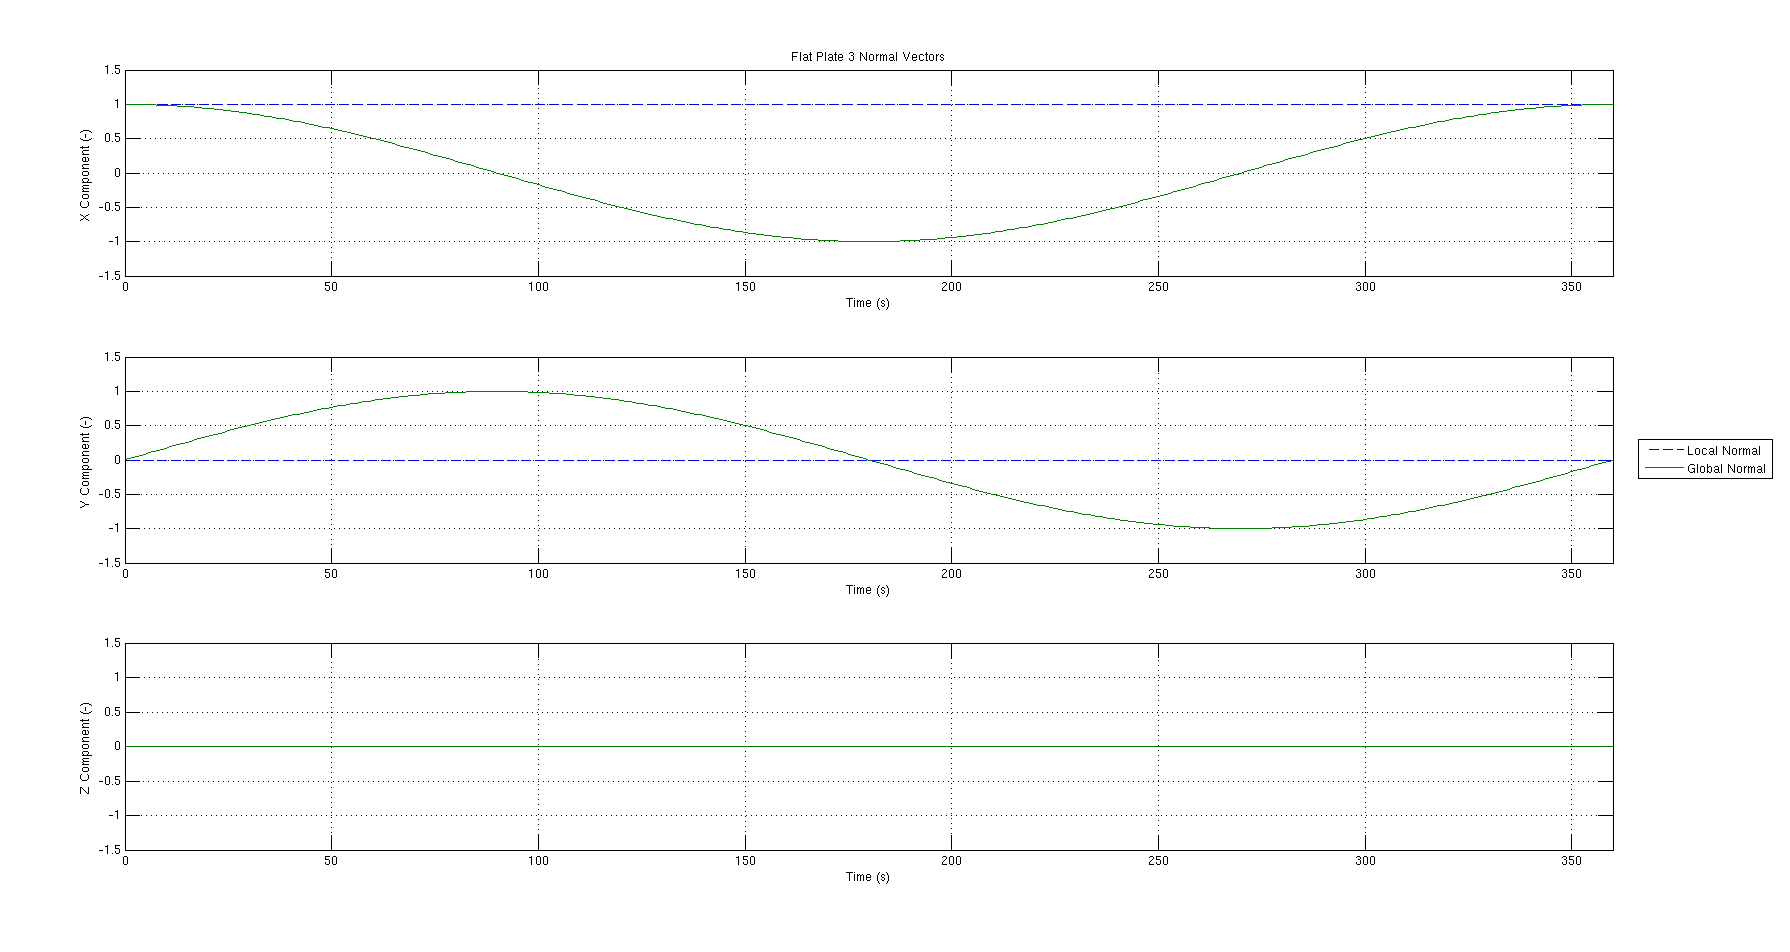
\includegraphics[height=90mm]{figs/art_test_0.png}
\caption{FlatPlate 3's Local and ``Global" Normal}
\label{fig:artic_normal_3}
\end{center}
\end{figure}

Similarly, FlatPlate 4's local normal stays in the negative X direction, and
the ``global" normal rotates through the X-Y plane in a counter-clockwise
manner, returning to its original position at the end of the simulation.
This behavior is shown below in Figure \ref{fig:artic_normal_4}.

\begin{figure}[H]
\begin{center}
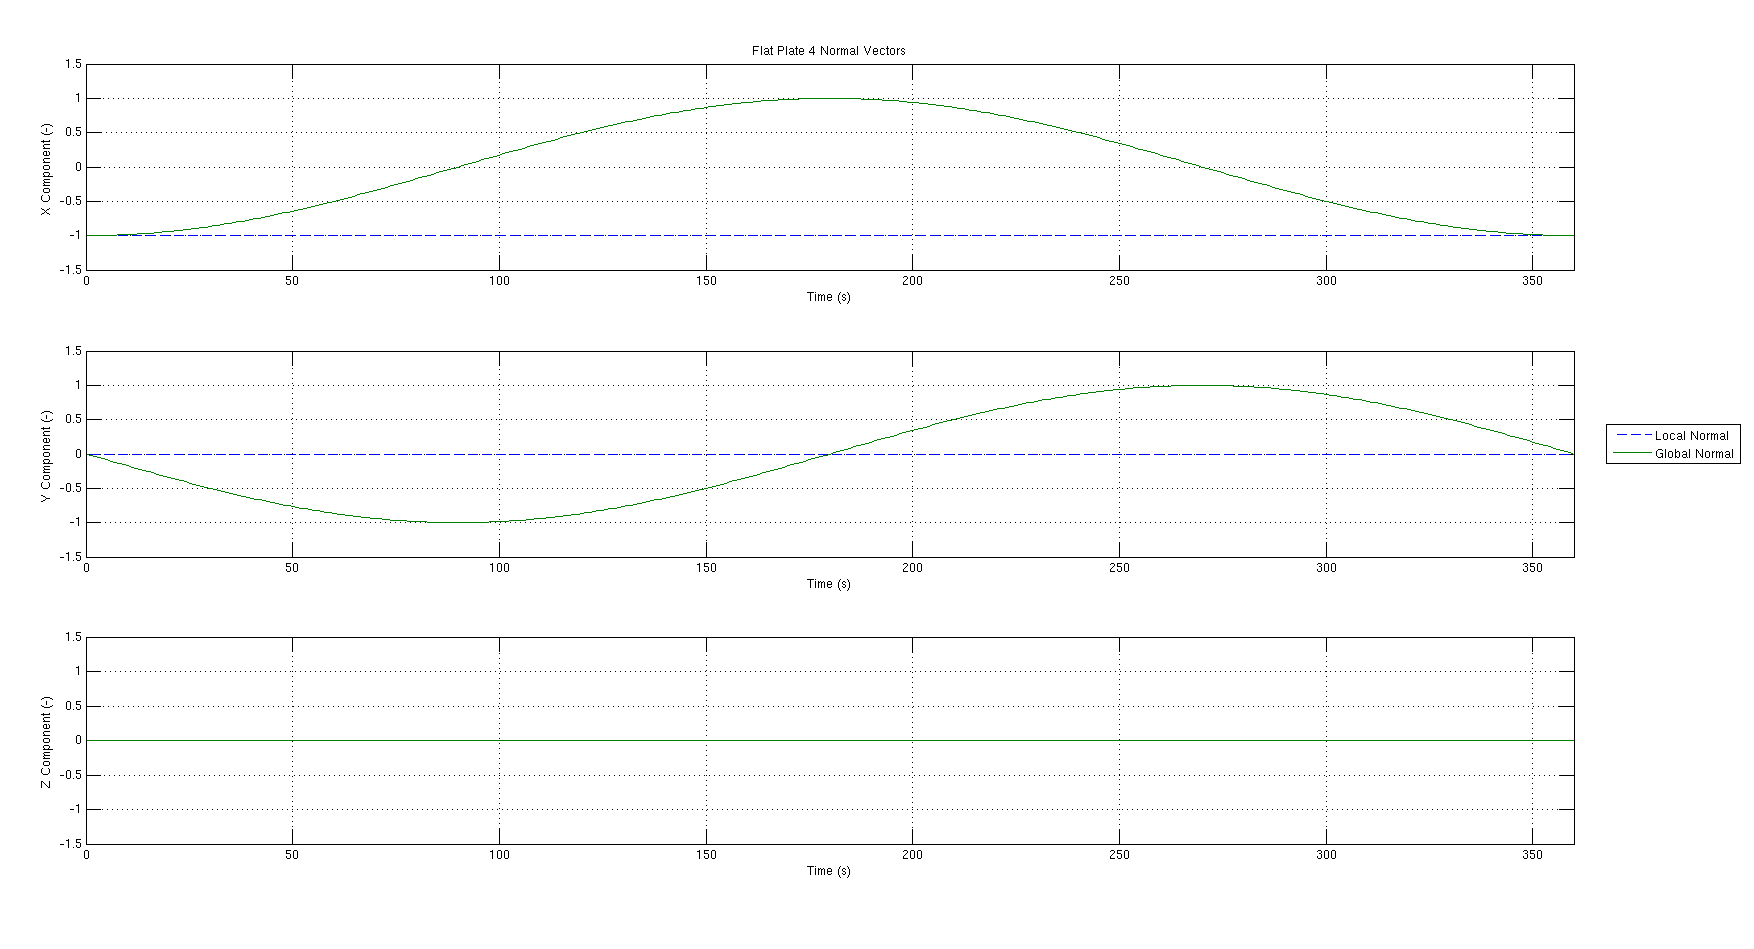
\includegraphics[height=90mm]{figs/art_test_1.png}
\caption{FlatPlate 4's Local and ``Global" Normal}
\label{fig:artic_normal_4}
\end{center}
\end{figure}

FlatPlate 5 and 6's local positions stays constant at the origin. Their
``global" positions move in the manner described in Equations \ref{position_equation_1},
\ref{position_equation_2}, and \ref{position_equation_3}.
as shown in Figures \ref{fig:artic_position_5} and \ref{fig:artic_position_6}, shown
below.

\begin{figure}[H]
\begin{center}
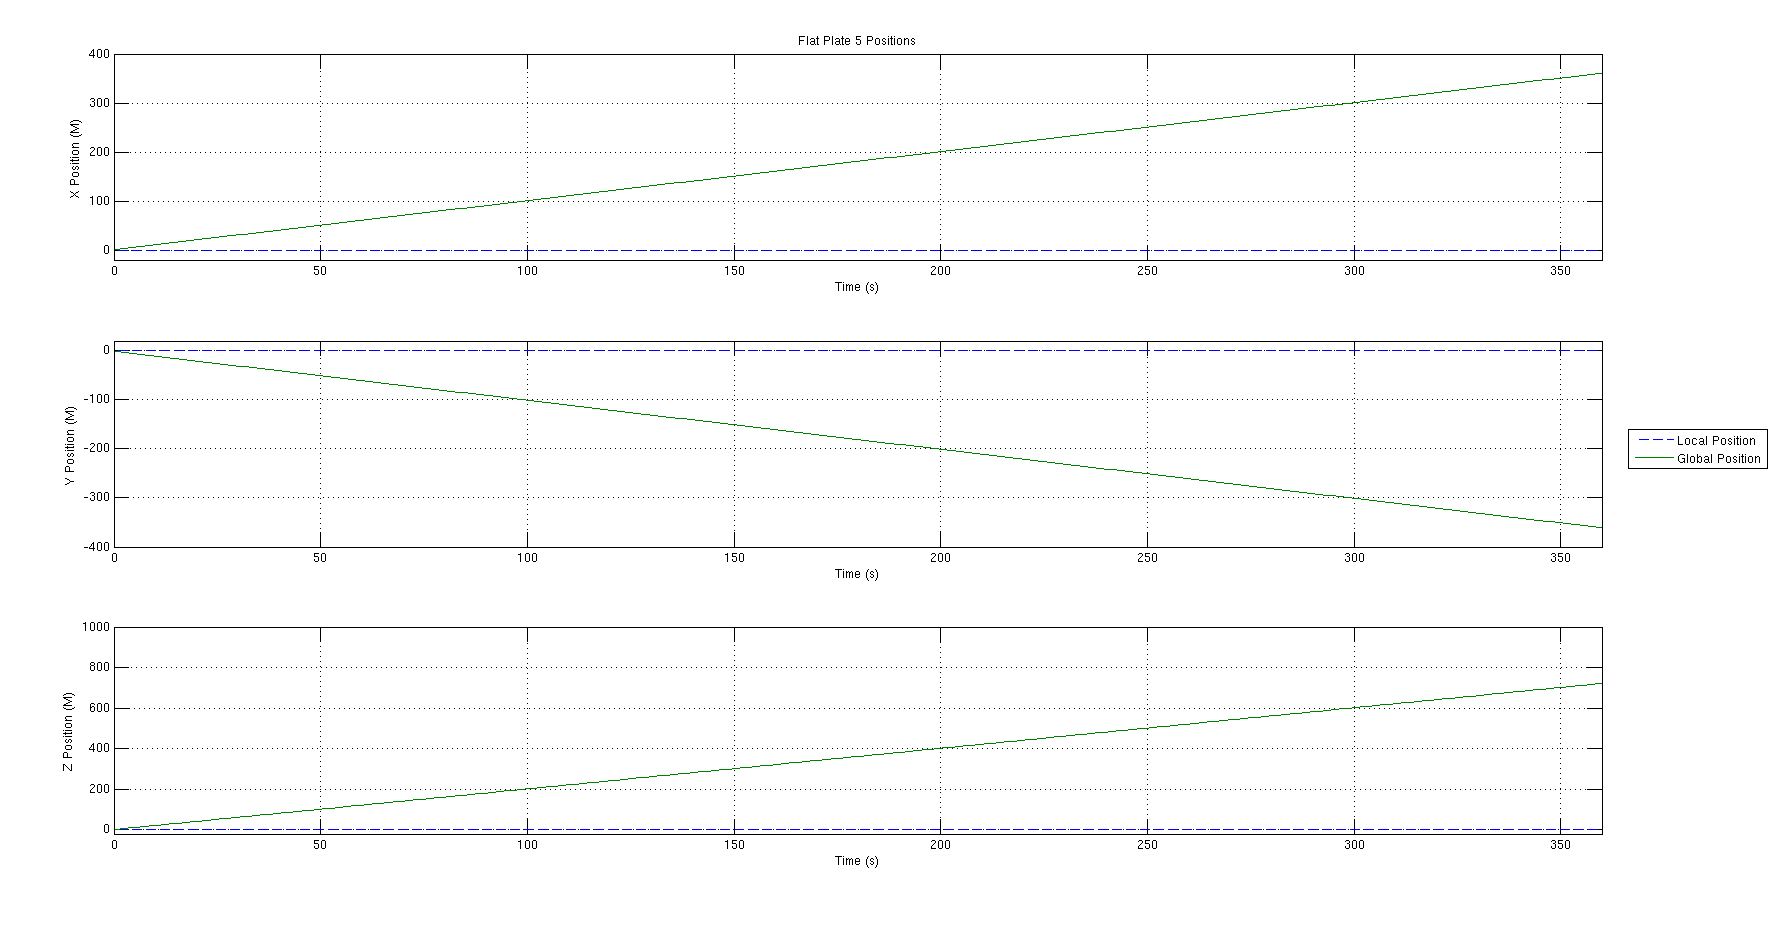
\includegraphics[height=90mm]{figs/art_test_2.png}
\caption{FlatPlate 5's Local and ``Global" Position}
\label{fig:artic_position_5}
\end{center}
\end{figure}

\begin{figure}[H]
\begin{center}
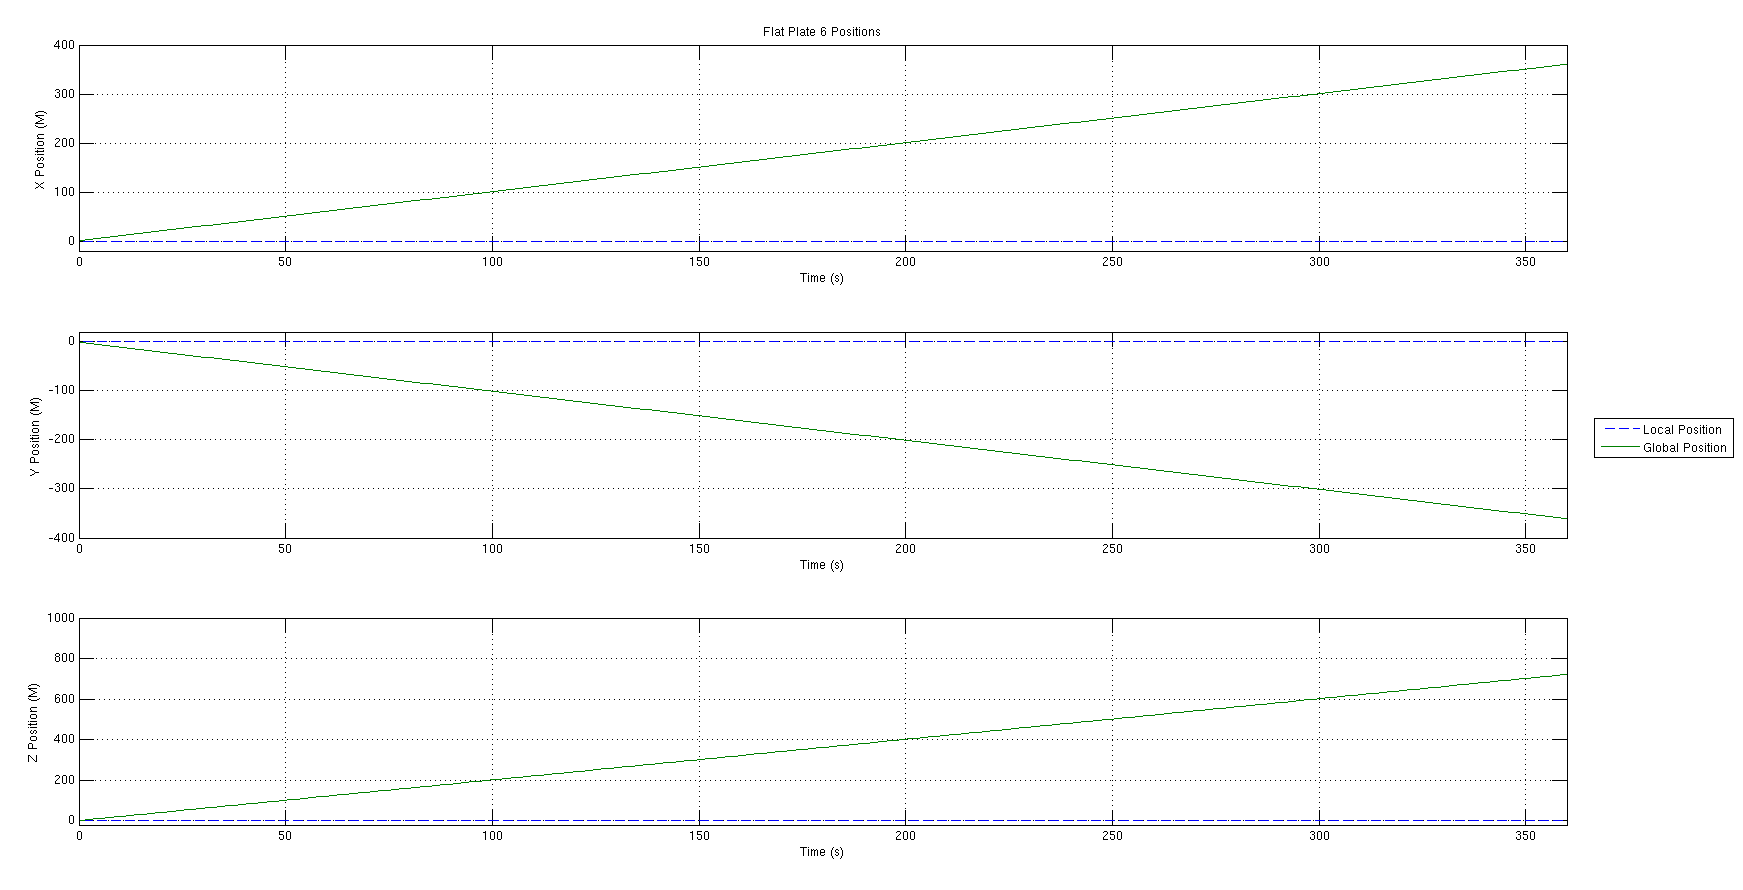
\includegraphics[height=90mm]{figs/art_test_3.png}
\caption{FlatPlate 6's Local and ``Global" Position}
\label{fig:artic_position_6}
\end{center}
\end{figure}

All behavior is qualitatively as expected, which demonstrates the articuation feature of
the \ModelDesc.

\end{description}

\test{Articulation Test, Configuration 1}\label{test:art_test_1}

\begin{description}

\item[] \ \newline

The goal of the following tests is to demonstrate the correct relative state
computations of FlatPlates associated with MassBody objects that
have been placed in various configurations. For these tests,
the following configuration will be used.

\begin{figure}[H]
\begin{center}
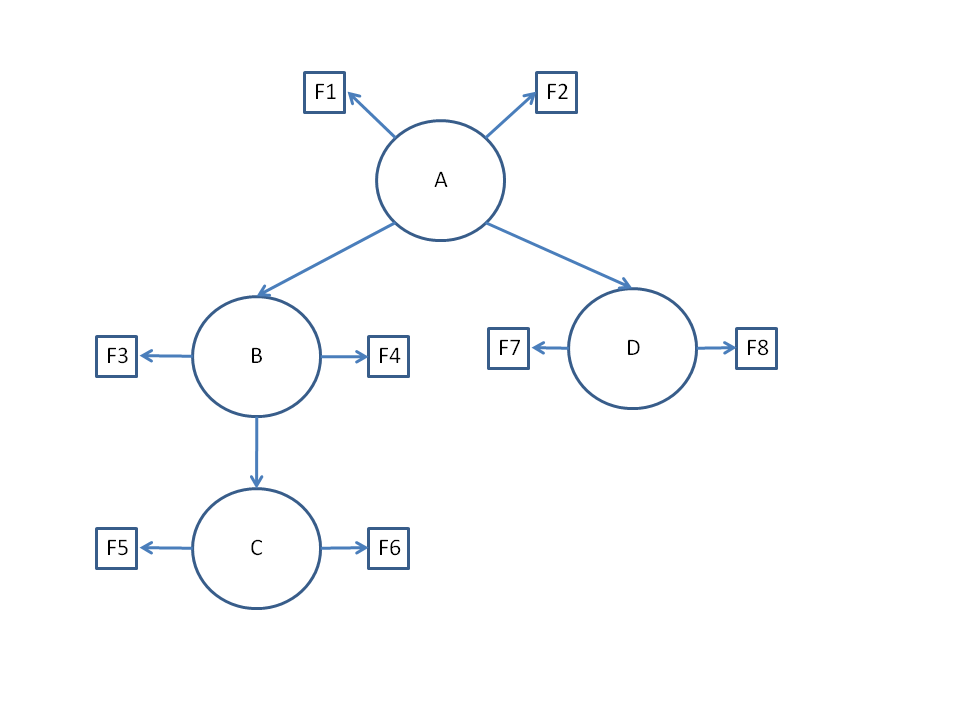
\includegraphics[height=100mm]{figs/art_figure.png}
\caption{The MassBody and FlatPlate configuration for Articulation
Validation Testing}
\label{fig:artic_config_1}
\end{center}
\end{figure}

Figure \ref{fig:artic_config_1} shows this configuration. Four MassBody
objects are used, labeled A through D. MassBody B is a child of
MassBody A. MassBody C is a child of MassBody B. MassBody D is
a child of MassBody A. Each child body will have a position and
orientation (in the form of a rotation matrix) defined. Further information
about these definitions can be found in the MassBody documentation
\cite{dynenv:MASS}.

This configuration also involves eight FlatPlate objects, labeled as
F1 - F8 in Figure \ref{fig:artic_config_1}. FlatPlates 1 and 2 are
attached to MassBody A. FlatPlates 3 and 4 are attached to MassBody B.
FlatPlates 5 and 6 are attached to MassBody C, and FlatPlates 7 and 8
are attached to MassBody D. Each FlatPlate will have its position and
normal defined with respect to its attached MassBody's structural
reference frame.

The six tests that follow will use this configuration of MassBodys
and FlatPlates. All tests will randomly position and orient MassBodys
with respect to their parent, and each FlatPlate with respect to
the appropriate MassBody. A final, "global" MassBody structural frame will
then be selected, and the position and orientation of all FlatPlates
relative to this "global" structural frame will be computed using the
articulation feature. These results will then be compared to an
independently programmed Matlab solution.

Note that all random relative positions and orientations were created in Matlab,
and the states themselves will be presented with each test.

\begin{itemize}
\item{$x_{A:B}$}: (Location of MassBody B's
structural origin in MassBody A's structural coordinates.)
\item{$T_{A:B}$}: (The transformation matrix from MassBody
A's structural reference frame to MassBody B's structural reference frame.)
\item{$x_{A:Fn}$}: (FlatPlate n's position defined in MassBody A's structural
reference frame.)
\item{$\hat{x}_{A:Fn}$}: (FlatPlate n's normal defined in MassBody A's structural
reference frame.)
\end{itemize}

\item[Purpose:] \ \newline
SIM directory: SIM\_ARTICULATION
RUN directory: SET\_test/RUN\_articulation\_1

The purpose of this test is to demonstrate the relative state calculation
between mass body structural frames, which is used by the articulation
feature.

\item[Requirements:] \ \newline

By passing this test, the \ModelDesc partially satisfies
the requirement \traceref{reqt:surfacemodel_artic}

\item[Procedure:] \ \newline

The following relative positions and orientations were input for MassBodys
B, C and D, and for all FlatPlates, configured as shown in
\ref{fig:artic_config_1}.

$x_{A:B}$ = $\left( \begin{array} {ccc}    -2.0381 \\   -4.09991 \\    3.59179 
\end{array} \right)\\ \\$

$T_{A:B}$ = $\left( \begin{array} {ccc} 
   0.5738961762045672 & -0.6152633149134586 & 0.5404574287207816 \\ 
   0.6713942538549126 & 0.7313744132614041 & 0.119671314512468 \\ 
   -0.468906104490421 & 0.2941811022962542 & 0.8328172333852003 \\
\end{array} \right)\\ \\$

$x_{B:C}$ = $\left( \begin{array} {ccc}    1.40503 \\   -2.20043 \\   -2.63571 
\end{array} \right)\\ \\$

$T_{B:C}$ = $\left( \begin{array} {ccc} 
   0.1200730155375398 & 0.1674994268654244 & 0.9785327858275759 \\ 
   -0.9674416511940138 & -0.2014627819906493 & 0.1531972552221103 \\ 
   0.2227983897489432 & -0.9650682304751009 & 0.137855678348538 \\
\end{array} \right)\\ \\$

$x_{A:D}$ = $\left( \begin{array} {ccc}     3.4757 \\  -0.339964 \\   -1.27395 
\end{array} \right)\\ \\$

$T_{A:D}$ = $\left( \begin{array} {ccc} 
   0.8775360833103077 & 0.2816997479818719 & 0.3880408154760973 \\ 
   -0.3435153756221815 & 0.9339299286459263 & 0.0988538066569347 \\ 
   -0.3345558386869913 & -0.2200457687990501 & 0.9163254064108879 \\
\end{array} \right)\\ \\$

$x_{A:F1}$ = $\left( \begin{array} {ccc} 0.00575529 \\   -2.31225 \\    2.12175 
\end{array} \right)\\ \\$

$x_{A:F2}$ = $\left( \begin{array} {ccc}   -1.70562 \\    3.03695 \\  -0.958726 
\end{array} \right)\\ \\$

$x_{B:F3}$ = $\left( \begin{array} {ccc}   -2.73297 \\   -2.12864 \\   -3.22221 
\end{array} \right)\\ \\$

$x_{B:F4}$ = $\left( \begin{array} {ccc}    2.29363 \\   -3.30972 \\    3.85143 
\end{array} \right)\\ \\$

$x_{C:F5}$ = $\left( \begin{array} {ccc}    -1.3239 \\   -1.59037 \\   0.596073 
\end{array} \right)\\ \\$

$x_{C:F6}$ = $\left( \begin{array} {ccc}    1.09338 \\   0.528991 \\   0.548487 
\end{array} \right)\\ \\$

$x_{D:F7}$ = $\left( \begin{array} {ccc}  -0.694371 \\   -3.48133 \\    -0.4691 
\end{array} \right)\\ \\$

$x_{D:F8}$ = $\left( \begin{array} {ccc}   -2.93046 \\    1.31073 \\    0.22227 
\end{array} \right)\\ \\$

$\hat{x}_{A:F1}$ = $\left( \begin{array} {ccc}  -0.760258 \\   0.282587 \\  -0.584938 
\end{array} \right)\\ \\$

$\hat{x}_{A:F2}$ = $\left( \begin{array} {ccc}    0.69449 \\  -0.396341 \\   0.600498 
\end{array} \right)\\ \\$

$\hat{x}_{B:F3}$ = $\left( \begin{array} {ccc}  -0.273795 \\   0.820658 \\   0.501555 
\end{array} \right)\\ \\$

$\hat{x}_{B:F4}$ = $\left( \begin{array} {ccc}   0.046571 \\   -0.84212 \\   0.537275 
\end{array} \right)\\ \\$

$\hat{x}_{C:F5}$ = $\left( \begin{array} {ccc}     0.2905 \\    0.71079 \\   0.640615 
\end{array} \right)\\ \\$

$\hat{x}_{C:F6}$ = $\left( \begin{array} {ccc} -0.0100222 \\  -0.542243 \\   0.840162 
\end{array} \right)\\ \\$

$\hat{x}_{D:F7}$ = $\left( \begin{array} {ccc}   0.959905 \\   0.192204 \\    0.20406 
\end{array} \right)\\ \\$

$\hat{x}_{D:F8}$ = $\left( \begin{array} {ccc}   0.401064 \\   0.648818 \\   -0.64667 
\end{array} \right)\\ \\$

For this test, all FlatPlate positions and normals will be determined in
MassBody A's structural reference frame.

\item[Results:] \ \newline

The following are the results from the independently programmed Matlab solution:

$x_{A:F1}$  = $\left( \begin{array} {ccc} 0.005755290000000 \\ -2.312250000000000 \\ 2.121750000000000
\end{array} \right)\\ \\$

$\hat{x}_{A:F1}$  = $\left( \begin{array} {ccc} -0.760258000000000 \\ 0.282587000000000 \\ -0.584938000000000
\end{array} \right)\\ \\$

$x_{A:F2}$  = $\left( \begin{array} {ccc} -1.705620000000000 \\ 3.036950000000000 \\ -0.958726000000000
\end{array} \right)\\ \\$

$\hat{x}_{A:F2}$  = $\left( \begin{array} {ccc} 0.694490000000000 \\ -0.396341000000000 \\ 0.600498000000000                                                        
\end{array} \right)\\ \\$

$x_{A:F3}$  = $\left( \begin{array} {ccc} -3.524783758257438 \\ -4.923159938915734 \\ -0.823513103480981
\end{array} \right)\\ \\$

$\hat{x}_{A:F3}$  = $\left( \begin{array} {ccc} 0.158672960778442 \\ 0.916212285307206 \\ 0.367938327419081
\end{array} \right)\\ \\$

$x_{A:F4}$  = $\left( \begin{array} {ccc} -4.749880541258142 \\ -6.798722997227628 \\ 7.642858106345402
\end{array} \right)\\ \\$

$\hat{x}_{A:F4}$  = $\left( \begin{array} {ccc} -0.790599137524367 \\ -0.486502296998308 \\ 0.371843914602749
\end{array} \right)\\ \\$

$x_{A:F5}$  = $\left( \begin{array} {ccc} -0.242053578687549 \\ -9.056812083026088 \\ 1.439752668545422
\end{array} \right)\\ \\$

$\hat{x}_{A:F5}$  = $\left( \begin{array} {ccc} -0.997026104738064 \\ -0.065859729793698 \\ 0.040021179234804
\end{array} \right)\\ \\$

$x_{A:F6}$  = $\left( \begin{array} {ccc} -2.500561635645481 \\ -7.160482600091685 \\ 2.720484460501432
\end{array} \right)\\ \\$

$\hat{x}_{A:F6}$  = $\left( \begin{array} {ccc} -0.075122497880330 \\ -0.944778584252594 \\ 0.318982975777274
\end{array} \right)\\ \\$

$x_{A:F7}$  = $\left( \begin{array} {ccc} 4.219194918838575 \\ -3.683662944055208 \\ -2.317385259959287
\end{array} \right)\\ \\$

$\hat{x}_{A:F7}$  = $\left( \begin{array} {ccc} 0.708056780351428 \\ 0.405007525010866 \\ 0.578467778466478
\end{array} \right)\\ \\$

$x_{A:F8}$  = $\left( \begin{array} {ccc} 0.379497974748256 \\ 0.009746558872154 \\ -2.077845790037692
\end{array} \right)\\ \\$

$\hat{x}_{A:F8}$  = $\left( \begin{array} {ccc} 0.345416396940049 \\ 0.861227173478076 \\ -0.372792819818084
\end{array} \right)\\ \\$

All \ModelDesc articulation produced results are a numerical match to the
independently programmed Matlab solution.

\end{description}

\test{Articulation Test, Configuration 2}\label{test:art_test_2}

\begin{description}

\item[Purpose:] \ \newline
SIM directory: SIM\_ARTICULATION
RUN directory: SET\_test/RUN\_articulation\_2

The purpose of this test is to demonstrate the relative state calculation
between mass body structural frames, which is used by the articulation
feature.

\item[Requirements:] \ \newline

By passing this test, the \ModelDesc partially satisfies
the requirement \traceref{reqt:surfacemodel_artic}

\item[Procedure:] \ \newline

The following relative positions and orientations were input for MassBodys
B, C and D, and for all FlatPlates, configured as shown in
\ref{fig:artic_config_1}.

$x_{A:B}$ = $\left( \begin{array} {ccc}  0.0978881 \\    1.65429 \\   -2.12155
\end{array} \right)\\ \\$

$T_{A:B}$ = $\left( \begin{array} {ccc} 
   0.1908098464799607 & -0.6966135920642235 & -0.6916076241899547 \\ 
   0.04030743089433808 & 0.7095182653790713 & -0.703533326934959 \\ 
   0.9807991198512527 & 0.1063641595879615 & 0.1634617755138939 \\
\end{array} \right)\\ \\$

$x_{B:C}$ = $\left( \begin{array} {ccc}   -1.88698 \\    1.08009 \\   -3.95204
\end{array} \right)\\ \\$

$T_{B:C}$ = $\left( \begin{array} {ccc} 
   -0.7361133641239929 & -0.5508618941680473 & -0.3933043207385965 \\ 
   -0.4364024092758288 & -0.05791070693348288 & 0.897886010137543 \\ 
   -0.517387719545323 & 0.8325848446711333 & -0.197768612493578 \\
\end{array} \right)\\ \\$

$x_{A:D}$ = $\left( \begin{array} {ccc}    4.42141 \\    2.94013 \\  -0.773762
\end{array} \right)\\ \\$

$T_{A:D}$ = $\left( \begin{array} {ccc} 
   0.8222190420975497 & -0.3626722656735943 & 0.4386623696231186 \\ 
   0.04304325740965631 & 0.808117347462562 & 0.5874467045797761 \\ 
   -0.5675412978839106 & -0.4641284094313281 & 0.6800600670198124 \\
\end{array} \right)\\ \\$

$x_{A:F1}$ = $\left( \begin{array} {ccc}    3.39326 \\    2.47589 \\   0.948552
\end{array} \right)\\ \\$

$x_{A:F2}$ = $\left( \begin{array} {ccc}   -4.94456 \\ -0.00261188 \\   -4.32719
\end{array} \right)\\ \\$

$x_{B:F3}$ = $\left( \begin{array} {ccc}    -3.6932 \\    2.92994 \\   -1.23367
\end{array} \right)\\ \\$

$x_{B:F4}$ = $\left( \begin{array} {ccc}   -2.90045 \\  0.0849147 \\  -0.604298
\end{array} \right)\\ \\$

$x_{C:F5}$ = $\left( \begin{array} {ccc}    2.44785 \\   0.962552 \\   0.615419
\end{array} \right)\\ \\$

$x_{C:F6}$ = $\left( \begin{array} {ccc}   -2.22592 \\  -0.619661 \\    2.45179
\end{array} \right)\\ \\$

$x_{D:F7}$ = $\left( \begin{array} {ccc}  -0.528547 \\  -0.710206 \\   0.832302
\end{array} \right)\\ \\$

$x_{D:F8}$ = $\left( \begin{array} {ccc}    4.29469 \\    3.92779 \\    2.56689
\end{array} \right)\\ \\$

$\hat{x}_{A:F1}$ = $\left( \begin{array} {ccc}   0.768477 \\   0.607306 \\  -0.201548
\end{array} \right)\\ \\$

$\hat{x}_{A:F2}$ = $\left( \begin{array} {ccc}   0.741323 \\  -0.585104 \\  -0.328777
\end{array} \right)\\ \\$

$\hat{x}_{B:F3}$ = $\left( \begin{array} {ccc}   0.338868 \\  -0.512566 \\   0.788952
\end{array} \right)\\ \\$

$\hat{x}_{B:F4}$ = $\left( \begin{array} {ccc}    0.79904 \\   0.326973 \\   0.504603
\end{array} \right)\\ \\$

$\hat{x}_{C:F5}$ = $\left( \begin{array} {ccc}  -0.628147 \\   0.721774 \\  -0.290642
\end{array} \right)\\ \\$

$\hat{x}_{C:F6}$ = $\left( \begin{array} {ccc}   0.772102 \\   0.554193 \\   0.311013
\end{array} \right)\\ \\$

$\hat{x}_{D:F7}$ = $\left( \begin{array} {ccc}   0.360979 \\    0.56045 \\   0.745379
\end{array} \right)\\ \\$

$\hat{x}_{D:F8}$ = $\left( \begin{array} {ccc} -0.0567124 \\  -0.673532 \\  -0.736979
\end{array} \right)\\ \\$

For this test, all FlatPlate positions and normals will be determined in
MassBody A's structural reference frame.

\item[Results:] \ \newline

The following are the results from the independently programmed Matlab solution:

$x_{A:F1}$  = $\left( \begin{array} {ccc} 3.393260000000000 \\ 2.475890000000000 \\ 0.948552000000000
\end{array} \right)\\ \\$

$\hat{x}_{A:F1}$  = $\left( \begin{array} {ccc} 0.768477000000000 \\ 0.607306000000000 \\ -0.201548000000000
\end{array} \right)\\ \\$

$x_{A:F2}$  = $\left( \begin{array} {ccc} -4.944560000000000 \\ -0.002611880000000 \\ -4.327190000000000
\end{array} \right)\\ \\$

$\hat{x}_{A:F2}$  = $\left( \begin{array} {ccc} 0.741323000000000 \\ -0.585104000000000 \\ -0.328777000000000
\end{array} \right)\\ \\$

$x_{A:F3}$  = $\left( \begin{array} {ccc} -1.698694921132129 \\ 6.174650991917465 \\ -1.830273046859699
\end{array} \right)\\ \\$

$\hat{x}_{A:F3}$  = $\left( \begin{array} {ccc} 0.817802559638069 \\ -0.515818777492667 \\ 0.255207065574980
\end{array} \right)\\ \\$

$x_{A:F4}$  = $\left( \begin{array} {ccc} -1.044818572348511 \\ 3.670755774841175 \\ -0.274096611834425
\end{array} \right)\\ \\$

$\hat{x}_{A:F4}$  = $\left( \begin{array} {ccc} 0.660558319607464 \\ -0.270957134796642 \\ -0.700175256231008
\end{array} \right)\\ \\$

$x_{A:F5}$  = $\left( \begin{array} {ccc} -4.831430641784406 \\ 4.428271095306710 \\ 0.125952487453193
\end{array} \right)\\ \\$

$\hat{x}_{A:F5}$  = $\left( \begin{array} {ccc} 0.993640457587366 \\ -0.061953197643265 \\ -0.094019015078572
\end{array} \right)\\ \\$

$x_{A:F6}$  = $\left( \begin{array} {ccc} -4.002062137405464 \\ 5.194819674814850 \\ -5.016452941828739
\end{array} \right)\\ \\$

$\hat{x}_{A:F6}$  = $\left( \begin{array} {ccc} -0.063419258454724 \\ 0.549761951194300 \\ 0.832910715802174
\end{array} \right)\\ \\$

$x_{A:F7}$  = $\left( \begin{array} {ccc} 3.483893254973209 \\ 2.171594545706472 \\ -0.856808499849251
\end{array} \right)\\ \\$

$\hat{x}_{A:F7}$  = $\left( \begin{array} {ccc} -0.102105963862838 \\ -0.023959274098709 \\ 0.994484901801080
\end{array} \right)\\ \\$

$x_{A:F8}$  = $\left( \begin{array} {ccc} 6.664834691801769 \\ 3.365313710639066 \\ 5.163163569410596
\end{array} \right)\\ \\$

$\hat{x}_{A:F8}$  = $\left( \begin{array} {ccc} 0.342644991720493 \\ -0.181671987617076 \\ -0.921731737732234
\end{array} \right)\\ \\$

All \ModelDesc articulation produced results are a numerical match to the
independently programmed Matlab solution.


\end{description}

\test{Articulation Test, Configuration 3}\label{test:art_test_3}

\begin{description}

\item[Purpose:] \ \newline
SIM directory: SIM\_ARTICULATION
RUN directory: SET\_test/RUN\_articulation\_3

The purpose of this test is to demonstrate the relative state calculation
between mass body structural frames, which is used by the articulation
feature.

\item[Requirements:] \ \newline

By passing this test, the \ModelDesc partially satisfies
the requirement \traceref{reqt:surfacemodel_artic}

\item[Procedure:] \ \newline

The following relative positions and orientations were input for MassBodys
B, C and D, and for all FlatPlates, configured as shown in
\ref{fig:artic_config_1}.

$x_{A:B}$ = $\left( \begin{array} {ccc}  -0.126141 \\    4.21103 \\    2.79516
\end{array} \right)\\ \\$

$T_{A:B}$ = $\left( \begin{array} {ccc} 
   0.997369704807009 & 0.06997143703733257 & 0.01891216360204106 \\
   -0.07007880132551818 & 0.9975285522158546 & 0.005074358966393988 \\
   -0.01851036298829154 & -0.006386353660100277 & 0.99980827209469 \\
\end{array} \right)\\ \\$
             
$x_{B:C}$ = $\left( \begin{array} {ccc}    2.69991 \\    3.53459 \\    4.99746
\end{array} \right)\\ \\$

$T_{B:C}$ = $\left( \begin{array} {ccc} 
   -0.07082185013447745 & 0.9972707676557767 & 0.02086340151527186 \\
   0.9728231355161533 & 0.06443288212731174 & 0.2224040258297676 \\
   0.2204527444783792 & 0.03604746426623952 & -0.9747313310712469 \\
\end{array} \right)\\ \\$
             
$x_{A:D}$ = $\left( \begin{array} {ccc}   -1.67924 \\  -0.878345 \\    1.04473
\end{array} \right)\\ \\$

$T_{A:D}$ = $\left( \begin{array} {ccc} 
   0.2629583935566351 & 0.4849501785352546 & -0.8340720637910962 \\ 
   -0.2381525060753064 & -0.8051199041282633 & -0.5431991566879935 \\
   -0.9349525480515922 & 0.3414751298632461 & -0.09622093627020228 \\
\end{array} \right)\\ \\$
             
$x_{A:F1}$ = $\left( \begin{array} {ccc}   -1.49968 \\   0.670615 \\    1.06301
\end{array} \right)\\ \\$
              
$x_{A:F2}$ = $\left( \begin{array} {ccc}    2.28029 \\   0.508347 \\    4.97695
\end{array} \right)\\ \\$
              
$x_{B:F3}$ = $\left( \begin{array} {ccc}     3.8862 \\   -4.52567 \\    2.66886
\end{array} \right)\\ \\$
              
$x_{B:F4}$ = $\left( \begin{array} {ccc}    3.64855 \\   -3.53627 \\   -3.90689
\end{array} \right)\\ \\$
              
$x_{C:F5}$ = $\left( \begin{array} {ccc}  -0.639442 \\    -2.7477 \\   -2.42615
\end{array} \right)\\ \\$
              
$x_{C:F6}$ = $\left( \begin{array} {ccc}   -3.61362 \\   0.551767 \\  -0.587464
\end{array} \right)\\ \\$
             
$x_{D:F7}$ = $\left( \begin{array} {ccc}  -0.431173 \\   -1.83218 \\   -1.84599
\end{array} \right)\\ \\$
              
$x_{D:F8}$ = $\left( \begin{array} {ccc}    1.14477 \\    -3.2097 \\     2.4224
\end{array} \right)\\ \\$
       
$\hat{x}_{A:F1}$ = $\left( \begin{array} {ccc}  -0.496347 \\  -0.260678 \\  -0.828062
\end{array} \right)\\ \\$

$\hat{x}_{A:F2}$ = $\left( \begin{array} {ccc}    0.12748 \\   0.820292 \\  -0.557557
\end{array} \right)\\ \\$

$\hat{x}_{B:F3}$ = $\left( \begin{array} {ccc}  -0.247273 \\   -0.23111 \\  -0.940981
\end{array} \right)\\ \\$

$\hat{x}_{B:F4}$ = $\left( \begin{array} {ccc}  -0.138757 \\   0.861377 \\  -0.488648
\end{array} \right)\\ \\$

$\hat{x}_{C:F5}$ = $\left( \begin{array} {ccc}    0.81173 \\  -0.130319 \\   0.569308
\end{array} \right)\\ \\$

$\hat{x}_{C:F6}$ = $\left( \begin{array} {ccc}   0.798565 \\  -0.347707 \\  -0.491318
\end{array} \right)\\ \\$

$\hat{x}_{D:F7}$ = $\left( \begin{array} {ccc}  -0.706014 \\  -0.123783 \\   0.697296
\end{array} \right)\\ \\$

$\hat{x}_{D:F8}$ = $\left( \begin{array} {ccc}    0.31147 \\  -0.909147 \\  -0.276475
\end{array} \right)\\ \\$

For this test, all FlatPlate positions and normals will be determined in
MassBody A's structural reference frame.

\item[Results:] \ \newline

The following are the results from the independently programmed Matlab solution:

$x_{A:F1}$  = $\left( \begin{array} {ccc} -1.499680000000000 \\ 0.670615000000000 \\ 1.063010000000000
\end{array} \right)\\ \\$

$\hat{x}_{A:F1}$  = $\left( \begin{array} {ccc} -0.496347000000000 \\ -0.260678000000000 \\ -0.828062000000000
\end{array} \right)\\ \\$

$x_{A:F2}$  = $\left( \begin{array} {ccc} 2.280290000000000 \\ 0.508347000000000 \\ 4.976950000000000
\end{array} \right)\\ \\$

$\hat{x}_{A:F2}$  = $\left( \begin{array} {ccc} 0.127480000000000 \\ 0.820292000000000 \\ -0.557557000000000
\end{array} \right)\\ \\$

$x_{A:F3}$  = $\left( \begin{array} {ccc} 4.017589108250925 \\ -0.048576328121540 \\ 5.514039881109446
\end{array} \right)\\ \\$

$\hat{x}_{A:F3}$  = $\left( \begin{array} {ccc} -0.213008787367317 \\ -0.241831433399704 \\ -0.946649790215024
\end{array} \right)\\ \\$

$x_{A:F4}$  = $\left( \begin{array} {ccc} 3.832947751292330 \\ 0.963744774509309 \\ -1.059923269035887
\end{array} \right)\\ \\$

$\hat{x}_{A:F4}$  = $\left( \begin{array} {ccc} -0.189711243925774 \\ 0.852659803976348 \\ -0.486807571524059
\end{array} \right)\\ \\$

$x_{A:F5}$  = $\left( \begin{array} {ccc} -0.896800453641627 \\ 6.761513732028066 \\ 9.536339519032627
\end{array} \right)\\ \\$

$\hat{x}_{A:F5}$  = $\left( \begin{array} {ccc} -0.105690202004579 \\ 0.819118589489993 \\ -0.563803645853018
\end{array} \right)\\ \\$

$x_{A:F6}$  = $\left( \begin{array} {ccc} 3.127969586147725 \\ 4.355819180534397 \\ 8.474810754421558
\end{array} \right)\\ \\$

$\hat{x}_{A:F6}$  = $\left( \begin{array} {ccc} -0.562542495689039 \\ 0.716526508239595 \\ 0.412474602529563
\end{array} \right)\\ \\$

$x_{A:F7}$  = $\left( \begin{array} {ccc} 0.369630753333818 \\ -0.242677512360114 \\ 2.577220871007037
\end{array} \right)\\ \\$

$\hat{x}_{A:F7}$  = $\left( \begin{array} {ccc} -0.808111747555158 \\ -0.004612216102558 \\ 0.589010901280250
\end{array} \right)\\ \\$

$x_{A:F8}$  = $\left( \begin{array} {ccc} -2.878644073458437 \\ 3.088194126743018 \\ 1.600330060734381
\end{array} \right)\\ \\$

$\hat{x}_{A:F8}$  = $\left( \begin{array} {ccc} 0.556910293004496 \\ 0.788610441057933 \\ 0.260662141351711
\end{array} \right)\\ \\$

All \ModelDesc articulation produced results are a numerical match to the
independently programmed Matlab solution.


\end{description}

\test{Articulation Test, Configuration 4}\label{test:art_test_4}

\begin{description}

\item[Purpose:] \ \newline
SIM directory: SIM\_ARTICULATION
RUN directory: SET\_test/RUN\_articulation\_4

The purpose of this test is to demonstrate the relative state calculation
between mass body structural frames, which is used by the articulation
feature.

\item[Requirements:] \ \newline

By passing this test, the \ModelDesc partially satisfies
the requirement \traceref{reqt:surfacemodel_artic}

\item[Procedure:] \ \newline

$x_{A:B}$ = $\left( \begin{array} {ccc}    -2.0381 \\   -4.09991 \\    3.59179 
\end{array} \right)\\ \\$

$T_{A:B}$ = $\left( \begin{array} {ccc} 
   0.5738961762045672 & -0.6152633149134586 & 0.5404574287207816 \\ 
   0.6713942538549126 & 0.7313744132614041 & 0.119671314512468 \\ 
   -0.468906104490421 & 0.2941811022962542 & 0.8328172333852003 \\
\end{array} \right)\\ \\$

$x_{B:C}$ = $\left( \begin{array} {ccc}    1.40503 \\   -2.20043 \\   -2.63571 
\end{array} \right)\\ \\$

$T_{B:C}$ = $\left( \begin{array} {ccc} 
   0.1200730155375398 & 0.1674994268654244 & 0.9785327858275759 \\ 
   -0.9674416511940138 & -0.2014627819906493 & 0.1531972552221103 \\ 
   0.2227983897489432 & -0.9650682304751009 & 0.137855678348538 \\
\end{array} \right)\\ \\$

$x_{A:D}$ = $\left( \begin{array} {ccc}     3.4757 \\  -0.339964 \\   -1.27395 
\end{array} \right)\\ \\$

$T_{A:D}$ = $\left( \begin{array} {ccc} 
   0.8775360833103077 & 0.2816997479818719 & 0.3880408154760973 \\ 
   -0.3435153756221815 & 0.9339299286459263 & 0.0988538066569347 \\ 
   -0.3345558386869913 & -0.2200457687990501 & 0.9163254064108879 \\
\end{array} \right)\\ \\$

$x_{A:F1}$ = $\left( \begin{array} {ccc} 0.00575529 \\   -2.31225 \\    2.12175 
\end{array} \right)\\ \\$

$x_{A:F2}$ = $\left( \begin{array} {ccc}   -1.70562 \\    3.03695 \\  -0.958726 
\end{array} \right)\\ \\$

$x_{B:F3}$ = $\left( \begin{array} {ccc}   -2.73297 \\   -2.12864 \\   -3.22221 
\end{array} \right)\\ \\$

$x_{B:F4}$ = $\left( \begin{array} {ccc}    2.29363 \\   -3.30972 \\    3.85143 
\end{array} \right)\\ \\$

$x_{C:F5}$ = $\left( \begin{array} {ccc}    -1.3239 \\   -1.59037 \\   0.596073 
\end{array} \right)\\ \\$

$x_{C:F6}$ = $\left( \begin{array} {ccc}    1.09338 \\   0.528991 \\   0.548487 
\end{array} \right)\\ \\$

$x_{D:F7}$ = $\left( \begin{array} {ccc}  -0.694371 \\   -3.48133 \\    -0.4691 
\end{array} \right)\\ \\$

$x_{D:F8}$ = $\left( \begin{array} {ccc}   -2.93046 \\    1.31073 \\    0.22227 
\end{array} \right)\\ \\$

$\hat{x}_{A:F1}$ = $\left( \begin{array} {ccc}  -0.760258 \\   0.282587 \\  -0.584938 
\end{array} \right)\\ \\$

$\hat{x}_{A:F2}$ = $\left( \begin{array} {ccc}    0.69449 \\  -0.396341 \\   0.600498 
\end{array} \right)\\ \\$

$\hat{x}_{B:F3}$ = $\left( \begin{array} {ccc}  -0.273795 \\   0.820658 \\   0.501555 
\end{array} \right)\\ \\$

$\hat{x}_{B:F4}$ = $\left( \begin{array} {ccc}   0.046571 \\   -0.84212 \\   0.537275 
\end{array} \right)\\ \\$

$\hat{x}_{C:F5}$ = $\left( \begin{array} {ccc}     0.2905 \\    0.71079 \\   0.640615 
\end{array} \right)\\ \\$

$\hat{x}_{C:F6}$ = $\left( \begin{array} {ccc} -0.0100222 \\  -0.542243 \\   0.840162 
\end{array} \right)\\ \\$

$\hat{x}_{D:F7}$ = $\left( \begin{array} {ccc}   0.959905 \\   0.192204 \\    0.20406 
\end{array} \right)\\ \\$

$\hat{x}_{D:F8}$ = $\left( \begin{array} {ccc}   0.401064 \\   0.648818 \\   -0.64667 
\end{array} \right)\\ \\$

The following relative positions and orientations were input for MassBodys
B, C and D, and for all FlatPlates, configured as shown in
\ref{fig:artic_config_1}.

For this test, all FlatPlate positions and normals will be determined in
MassBody B's structural reference frame.

\item[Results:] \ \newline

The following are the results from the independently programmed Matlab solution:

$x_{B:F1}$  = $\left( \begin{array} {ccc} -0.721414920408415 \\ 2.503759861841939 \\ -1.656755078610698
\end{array} \right)\\ \\$

$\hat{x}_{B:F1}$  = $\left( \begin{array} {ccc} -0.926308660941458 \\ -0.373756250695222 \\ -0.047525074519602
\end{array} \right)\\ \\$

$x_{B:F2}$  = $\left( \begin{array} {ccc} -6.659599317721549 \\ 4.898375725120448 \\ -1.846120705482019
\end{array} \right)\\ \\$

$\hat{x}_{B:F2}$  = $\left( \begin{array} {ccc} 0.966962837940397 \\ 0.248265314055368 \\ 0.057858450240594
\end{array} \right)\\ \\$

$x_{B:F3}$  = $\left( \begin{array} {ccc} -2.732970000000000 \\ -2.128640000000000 \\ -3.222210000000000
\end{array} \right)\\ \\$

$\hat{x}_{B:F3}$  = $\left( \begin{array} {ccc} -0.273795000000000 \\ 0.820658000000000 \\ 0.501555000000000
\end{array} \right)\\ \\$

$x_{B:F4}$  = $\left( \begin{array} {ccc} 2.293630000000000 \\ -3.309720000000000 \\ 3.851430000000000
\end{array} \right)\\ \\$

$\hat{x}_{B:F4}$  = $\left( \begin{array} {ccc} 0.046571000000000 \\ -0.842120000000000 \\ 0.537275000000000
\end{array} \right)\\ \\$

$x_{B:F5}$  = $\left( \begin{array} {ccc} 2.917459618112097 \\ -2.677033241976651 \\ -4.092657826184467
\end{array} \right)\\ \\$

$\hat{x}_{B:F5}$  = $\left( \begin{array} {ccc} -0.510038649789519 \\ -0.712776331772535 \\ 0.481467266707483
\end{array} \right)\\ \\$

$x_{B:F6}$  = $\left( \begin{array} {ccc} 1.146749527619891 \\ -2.653188853690494 \\ -1.409149805944291
\end{array} \right)\\ \\$

$\hat{x}_{B:F6}$  = $\left( \begin{array} {ccc} 0.710571808220327 \\ -0.703250584113397 \\ 0.022943911883140
\end{array} \right)\\ \\$

$x_{B:F7}$  = $\left( \begin{array} {ccc} 0.141278416984113 \\ 3.798385528453287 \\ -7.732894758882457
\end{array} \right)\\ \\$

$\hat{x}_{B:F7}$  = $\left( \begin{array} {ccc} 0.469802014524136 \\ 0.840823394154425 \\ 0.268891348378292
\end{array} \right)\\ \\$

$x_{B:F8}$  = $\left( \begin{array} {ccc} -4.205267465126678 \\ 3.950366275027509 \\ -4.646413544976000
\end{array} \right)\\ \\$

$\hat{x}_{B:F8}$  = $\left( \begin{array} {ccc} -0.533126985089867 \\ 0.817177495991682 \\ -0.219079382721772
\end{array} \right)\\ \\$

All \ModelDesc articulation produced results are a numerical match to the
independently programmed Matlab solution.


\end{description}

\test{Articulation Test, Configuration 5}\label{test:art_test_5}

\begin{description}

\item[Purpose:] \ \newline
SIM directory: SIM\_ARTICULATION
RUN directory: SET\_test/RUN\_articulation\_5

The purpose of this test is to demonstrate the relative state calculation
between mass body structural frames, which is used by the articulation
feature.

\item[Requirements:] \ \newline

By passing this test, the \ModelDesc partially satisfies
the requirement \traceref{reqt:surfacemodel_artic}

\item[Procedure:] \ \newline

The following relative positions and orientations were input for MassBodys
B, C and D, and for all FlatPlates, configured as shown in
\ref{fig:artic_config_1}.

$x_{A:B}$ = $\left( \begin{array} {ccc}    -2.0381 \\   -4.09991 \\    3.59179 
\end{array} \right)\\ \\$

$T_{A:B}$ = $\left( \begin{array} {ccc} 
   0.5738961762045672 & -0.6152633149134586 & 0.5404574287207816 \\ 
   0.6713942538549126 & 0.7313744132614041 & 0.119671314512468 \\ 
   -0.468906104490421 & 0.2941811022962542 & 0.8328172333852003 \\
\end{array} \right)\\ \\$

$x_{B:C}$ = $\left( \begin{array} {ccc}    1.40503 \\   -2.20043 \\   -2.63571 
\end{array} \right)\\ \\$

$T_{B:C}$ = $\left( \begin{array} {ccc} 
   0.1200730155375398 & 0.1674994268654244 & 0.9785327858275759 \\ 
   -0.9674416511940138 & -0.2014627819906493 & 0.1531972552221103 \\ 
   0.2227983897489432 & -0.9650682304751009 & 0.137855678348538 \\
\end{array} \right)\\ \\$

$x_{A:D}$ = $\left( \begin{array} {ccc}     3.4757 \\  -0.339964 \\   -1.27395 
\end{array} \right)\\ \\$

$T_{A:D}$ = $\left( \begin{array} {ccc} 
   0.8775360833103077 & 0.2816997479818719 & 0.3880408154760973 \\ 
   -0.3435153756221815 & 0.9339299286459263 & 0.0988538066569347 \\ 
   -0.3345558386869913 & -0.2200457687990501 & 0.9163254064108879 \\
\end{array} \right)\\ \\$

$x_{A:F1}$ = $\left( \begin{array} {ccc} 0.00575529 \\   -2.31225 \\    2.12175 
\end{array} \right)\\ \\$

$x_{A:F2}$ = $\left( \begin{array} {ccc}   -1.70562 \\    3.03695 \\  -0.958726 
\end{array} \right)\\ \\$

$x_{B:F3}$ = $\left( \begin{array} {ccc}   -2.73297 \\   -2.12864 \\   -3.22221 
\end{array} \right)\\ \\$

$x_{B:F4}$ = $\left( \begin{array} {ccc}    2.29363 \\   -3.30972 \\    3.85143 
\end{array} \right)\\ \\$

$x_{C:F5}$ = $\left( \begin{array} {ccc}    -1.3239 \\   -1.59037 \\   0.596073 
\end{array} \right)\\ \\$

$x_{C:F6}$ = $\left( \begin{array} {ccc}    1.09338 \\   0.528991 \\   0.548487 
\end{array} \right)\\ \\$

$x_{D:F7}$ = $\left( \begin{array} {ccc}  -0.694371 \\   -3.48133 \\    -0.4691 
\end{array} \right)\\ \\$

$x_{D:F8}$ = $\left( \begin{array} {ccc}   -2.93046 \\    1.31073 \\    0.22227 
\end{array} \right)\\ \\$

$\hat{x}_{A:F1}$ = $\left( \begin{array} {ccc}  -0.760258 \\   0.282587 \\  -0.584938 
\end{array} \right)\\ \\$

$\hat{x}_{A:F2}$ = $\left( \begin{array} {ccc}    0.69449 \\  -0.396341 \\   0.600498 
\end{array} \right)\\ \\$

$\hat{x}_{B:F3}$ = $\left( \begin{array} {ccc}  -0.273795 \\   0.820658 \\   0.501555 
\end{array} \right)\\ \\$

$\hat{x}_{B:F4}$ = $\left( \begin{array} {ccc}   0.046571 \\   -0.84212 \\   0.537275 
\end{array} \right)\\ \\$

$\hat{x}_{C:F5}$ = $\left( \begin{array} {ccc}     0.2905 \\    0.71079 \\   0.640615 
\end{array} \right)\\ \\$

$\hat{x}_{C:F6}$ = $\left( \begin{array} {ccc} -0.0100222 \\  -0.542243 \\   0.840162 
\end{array} \right)\\ \\$

$\hat{x}_{D:F7}$ = $\left( \begin{array} {ccc}   0.959905 \\   0.192204 \\    0.20406 
\end{array} \right)\\ \\$

$\hat{x}_{D:F8}$ = $\left( \begin{array} {ccc}   0.401064 \\   0.648818 \\   -0.64667 
\end{array} \right)\\ \\$

For this test, all FlatPlate positions and normals will be determined in
MassBody C's structural reference frame.

\item[Results:] \ \newline

The following are the results from the independently programmed Matlab solution:

$x_{C:F1}$  = $\left( \begin{array} {ccc} 1.490559938183432 \\ 1.259465415337173 \\ -4.878678195182763
\end{array} \right)\\ \\$

$\hat{x}_{C:F1}$  = $\left( \begin{array} {ccc} -0.220333475582930 \\ 0.964166843537344 \\ 0.147768604032725
\end{array} \right)\\ \\$

$x_{C:F2}$  = $\left( \begin{array} {ccc} 0.993340541039701 \\ 6.492876065883191 \\ -8.538768937726466
\end{array} \right)\\ \\$

$\hat{x}_{C:F2}$  = $\left( \begin{array} {ccc} 0.214306832176674 \\ -0.976632589653420 \\ -0.016179088177458
\end{array} \right)\\ \\$

$x_{C:F3}$  = $\left( \begin{array} {ccc} -1.058746833327544 \\ 3.898960349333953 \\ -1.072074340398352
\end{array} \right)\\ \\$

$\hat{x}_{C:F3}$  = $\left( \begin{array} {ccc} 0.595372364759175 \\ 0.176385492488708 \\ -0.783849844252446
\end{array} \right)\\ \\$

$x_{C:F4}$  = $\left( \begin{array} {ccc} 6.268770618632612 \\ 0.357624040424968 \\ 2.162808271756570
\end{array} \right)\\ \\$

$\hat{x}_{C:F4}$  = $\left( \begin{array} {ccc} 0.390278505560198 \\ 0.206910168131668 \\ 0.897145611641401
\end{array} \right)\\ \\$

$x_{C:F5}$  = $\left( \begin{array} {ccc} -1.323900000000000 \\ -1.590370000000000 \\ 0.596073000000000
\end{array} \right)\\ \\$

$\hat{x}_{C:F5}$  = $\left( \begin{array} {ccc} 0.290500000000000 \\ 0.710790000000000 \\ 0.640615000000000
\end{array} \right)\\ \\$

$x_{C:F6}$  = $\left( \begin{array} {ccc} 1.093380000000000 \\ 0.528991000000000 \\ 0.548487000000000
\end{array} \right)\\ \\$

$\hat{x}_{C:F6}$  = $\left( \begin{array} {ccc} -0.010022200000000 \\ -0.542243000000000 \\ 0.840162000000000
\end{array} \right)\\ \\$

$x_{C:F7}$  = $\left( \begin{array} {ccc} -4.134706702562834 \\ -0.766806861259732 \\ -6.773503967333159
\end{array} \right)\\ \\$

$\hat{x}_{C:F7}$  = $\left( \begin{array} {ccc} 0.460366981418975 \\ -0.582707240290149 \\ -0.669712613569149
\end{array} \right)\\ \\$

$x_{C:F8}$  = $\left( \begin{array} {ccc} -1.610929825206028 \\ 3.880444650171289 \\ -7.463090219546920
\end{array} \right)\\ \\$

$\hat{x}_{C:F8}$  = $\left( \begin{array} {ccc} -0.141513761230369 \\ 0.317576038920061 \\ -0.937613210767787
\end{array} \right)\\ \\$

All \ModelDesc articulation produced results are a numerical match to the
independently programmed Matlab solution.


\end{description}

\test{Articulation Test, Configuration 6}\label{test:art_test_6}

\begin{description}

\item[Purpose:] \ \newline
SIM directory: SIM\_ARTICULATION
RUN directory: SET\_test/RUN\_articulation\_6

The purpose of this test is to demonstrate the relative state calculation
between mass body structural frames, which is used by the articulation
feature.

Note also that the standard notation for relative states used in the
Reference Frame documentation \cite{dynenv:REFFRAMES} will be
followed here. The salient
pieces are as follows:

\item[Requirements:] \ \newline

By passing this test, the \ModelDesc partially satisfies
the requirement \traceref{reqt:surfacemodel_artic}

\item[Procedure:] \ \newline

The following relative positions and orientations were input for MassBodys
B, C and D, and for all FlatPlates, configured as shown in
\ref{fig:artic_config_1}.

$x_{A:B}$ = $\left( \begin{array} {ccc}    -2.0381 \\   -4.09991 \\    3.59179 
\end{array} \right)\\ \\$

$T_{A:B}$ = $\left( \begin{array} {ccc} 
   0.5738961762045672 & -0.6152633149134586 & 0.5404574287207816 \\ 
   0.6713942538549126 & 0.7313744132614041 & 0.119671314512468 \\ 
   -0.468906104490421 & 0.2941811022962542 & 0.8328172333852003 \\
\end{array} \right)\\ \\$

$x_{B:C}$ = $\left( \begin{array} {ccc}    1.40503 \\   -2.20043 \\   -2.63571 
\end{array} \right)\\ \\$

$T_{B:C}$ = $\left( \begin{array} {ccc} 
   0.1200730155375398 & 0.1674994268654244 & 0.9785327858275759 \\ 
   -0.9674416511940138 & -0.2014627819906493 & 0.1531972552221103 \\ 
   0.2227983897489432 & -0.9650682304751009 & 0.137855678348538 \\
\end{array} \right)\\ \\$

$x_{A:D}$ = $\left( \begin{array} {ccc}     3.4757 \\  -0.339964 \\   -1.27395 
\end{array} \right)\\ \\$

$T_{A:D}$ = $\left( \begin{array} {ccc} 
   0.8775360833103077 & 0.2816997479818719 & 0.3880408154760973 \\ 
   -0.3435153756221815 & 0.9339299286459263 & 0.0988538066569347 \\ 
   -0.3345558386869913 & -0.2200457687990501 & 0.9163254064108879 \\
\end{array} \right)\\ \\$

$x_{A:F1}$ = $\left( \begin{array} {ccc} 0.00575529 \\   -2.31225 \\    2.12175 
\end{array} \right)\\ \\$

$x_{A:F2}$ = $\left( \begin{array} {ccc}   -1.70562 \\    3.03695 \\  -0.958726 
\end{array} \right)\\ \\$

$x_{B:F3}$ = $\left( \begin{array} {ccc}   -2.73297 \\   -2.12864 \\   -3.22221 
\end{array} \right)\\ \\$

$x_{B:F4}$ = $\left( \begin{array} {ccc}    2.29363 \\   -3.30972 \\    3.85143 
\end{array} \right)\\ \\$

$x_{C:F5}$ = $\left( \begin{array} {ccc}    -1.3239 \\   -1.59037 \\   0.596073 
\end{array} \right)\\ \\$

$x_{C:F6}$ = $\left( \begin{array} {ccc}    1.09338 \\   0.528991 \\   0.548487 
\end{array} \right)\\ \\$

$x_{D:F7}$ = $\left( \begin{array} {ccc}  -0.694371 \\   -3.48133 \\    -0.4691 
\end{array} \right)\\ \\$

$x_{D:F8}$ = $\left( \begin{array} {ccc}   -2.93046 \\    1.31073 \\    0.22227 
\end{array} \right)\\ \\$

$\hat{x}_{A:F1}$ = $\left( \begin{array} {ccc}  -0.760258 \\   0.282587 \\  -0.584938 
\end{array} \right)\\ \\$

$\hat{x}_{A:F2}$ = $\left( \begin{array} {ccc}    0.69449 \\  -0.396341 \\   0.600498 
\end{array} \right)\\ \\$

$\hat{x}_{B:F3}$ = $\left( \begin{array} {ccc}  -0.273795 \\   0.820658 \\   0.501555 
\end{array} \right)\\ \\$

$\hat{x}_{B:F4}$ = $\left( \begin{array} {ccc}   0.046571 \\   -0.84212 \\   0.537275 
\end{array} \right)\\ \\$

$\hat{x}_{C:F5}$ = $\left( \begin{array} {ccc}     0.2905 \\    0.71079 \\   0.640615 
\end{array} \right)\\ \\$

$\hat{x}_{C:F6}$ = $\left( \begin{array} {ccc} -0.0100222 \\  -0.542243 \\   0.840162 
\end{array} \right)\\ \\$

$\hat{x}_{D:F7}$ = $\left( \begin{array} {ccc}   0.959905 \\   0.192204 \\    0.20406 
\end{array} \right)\\ \\$

$\hat{x}_{D:F8}$ = $\left( \begin{array} {ccc}   0.401064 \\   0.648818 \\   -0.64667 
\end{array} \right)\\ \\$

For this test, all FlatPlate positions and normals will be determined in
MassBody D's structural reference frame.

\item[Results:] \ \newline

The following are the results from the independently programmed Matlab solution:

$x_{D:F1}$  = $\left( \begin{array} {ccc} -2.282923962152712 \\ -0.314319691540555 \\ 4.706449634362594
\end{array} \right)\\ \\$

$\hat{x}_{D:F1}$  = $\left( \begin{array} {ccc} -0.814528959465332 \\ 0.467253421227741 \\ -0.343826871434294
\end{array} \right)\\ \\$

$x_{D:F2}$  = $\left( \begin{array} {ccc} -3.473199658403271 \\ 4.964825229431776 \\ 1.279212980717872
\end{array} \right)\\ \\$

$\hat{x}_{D:F2}$  = $\left( \begin{array} {ccc} 0.730808608295058 \\ -0.549361201875428 \\ 0.405119049540781
\end{array} \right)\\ \\$

$x_{D:F3}$  = $\left( \begin{array} {ccc} -7.259474338796993 \\ -1.831082646567445 \\ 3.763312361159124
\end{array} \right)\\ \\$

$\hat{x}_{D:F3}$  = $\left( \begin{array} {ccc} 0.540113107014310 \\ 0.837543576798951 \\ 0.082457635232693
\end{array} \right)\\ \\$

$x_{D:F4}$  = $\left( \begin{array} {ccc} -5.577589023893677 \\ -2.324954515539580 \\ 12.343836397635599
\end{array} \right)\\ \\$

$\hat{x}_{D:F4}$  = $\left( \begin{array} {ccc} -0.686536229216390 \\ -0.146017909387756 \\ 0.712282355654953
\end{array} \right)\\ \\$

$x_{D:F5}$  = $\left( \begin{array} {ccc} -4.664969425877037 \\ -6.595559952223573 \\ 5.648536405116573
\end{array} \right)\\ \\$

$\hat{x}_{D:F5}$  = $\left( \begin{array} {ccc} -0.877949201168424 \\ 0.284941670041608 \\ 0.384725482866194
\end{array} \right)\\ \\$

$x_{D:F6}$  = $\left( \begin{array} {ccc} -5.615719993914686 \\ -3.922083637064444 \\ 7.160421263092290
\end{array} \right)\\ \\$

$\hat{x}_{D:F6}$  = $\left( \begin{array} {ccc} -0.208288177597411 \\ -0.825018581285846 \\ 0.525319405116621
\end{array} \right)\\ \\$

$x_{D:F7}$  = $\left( \begin{array} {ccc} -0.694371000000000 \\ -3.481330000000000 \\ -0.469100000000000
\end{array} \right)\\ \\$

$\hat{x}_{D:F7}$  = $\left( \begin{array} {ccc} 0.959905000000000 \\ 0.192204000000000 \\ 0.204060000000000
\end{array} \right)\\ \\$

$x_{D:F8}$  = $\left( \begin{array} {ccc} -2.930460000000000 \\ 1.310730000000000 \\ 0.222270000000000
\end{array} \right)\\ \\$

$\hat{x}_{D:F8}$  = $\left( \begin{array} {ccc} 0.401064000000000 \\ 0.648818000000000 \\ -0.646670000000000
\end{array} \right)\\ \\$

All \ModelDesc articulation produced results are a numerical match to the
independently programmed Matlab solution.


\end{description}

\newpage

\boilerplatetraceability

\newpage
\boilerplatemetrics
